\documentclass[11pt,a4paper,oneside,openany]{report}
\usepackage{fontspec,xeCJK,geometry,xcolor,graphicx,amsmath,amssymb,array,booktabs,tabularx,fancyhdr,float,placeins,needspace,hyperref,fvextra}
\geometry{left=25mm,right=23mm,top=22mm,bottom=22mm,headheight=15pt,headsep=6mm}
\setmainfont{Times New Roman}\setsansfont{Segoe UI}\setmonofont{Consolas}
\setCJKmainfont[BoldFont=SimHei]{SimSun}\setCJKsansfont{Microsoft YaHei}\setCJKmonofont{Microsoft YaHei}
\definecolor{navy}{HTML}{203A4C}
\hypersetup{colorlinks=true,linkcolor=navy,urlcolor=navy,citecolor=navy,bookmarksnumbered=true,pdftitle={可核验教学智能体研究：数据、偏好优化与记忆},pdfauthor={Verifiable Tutoring Lab}}
\renewcommand{\contentsname}{目录}\renewcommand{\bibname}{参考文献}\renewcommand{\figurename}{图}\renewcommand{\tablename}{表}
\setcounter{tocdepth}{1}\setcounter{secnumdepth}{2}
\pagestyle{fancy}\fancyhf{}\fancyhead[L]{\small 可核验教学智能体研究}\fancyhead[R]{\small 研究报告与学习注释}\fancyfoot[C]{\small\thepage}
\renewcommand{\headrulewidth}{0.3pt}
\setlength{\parindent}{2em}\setlength{\parskip}{3pt}\linespread{1.1}
\setlength{\emergencystretch}{3em}
\clubpenalty=10000\widowpenalty=10000\displaywidowpenalty=10000
\setlength{\textfloatsep}{11pt}\setlength{\intextsep}{10pt}\setlength{\tabcolsep}{4.5pt}
\renewcommand{\topfraction}{0.9}\renewcommand{\bottomfraction}{0.8}\renewcommand{\textfraction}{0.08}\renewcommand{\floatpagefraction}{0.8}
\newcolumntype{Y}{>{\raggedright\arraybackslash}X}\renewcommand{\arraystretch}{1.14}\raggedbottom
\RecustomVerbatimEnvironment{verbatim}{Verbatim}{fontsize=\small,breaklines=true,breakanywhere=true,breaksymbolleft={\tiny\texttt{>}},breaksymbolright={}}
\newcommand{\filepath}[1]{\path{#1}}
\newcommand{\sourcefilename}[1]{\texttt{\detokenize{#1}}}
\newcommand{\chapterprefix}{第\thechapter 章}
\makeatletter
\def\@makechapterhead#1{\vspace*{2mm}{\parindent\z@\raggedright\normalfont{\small\sffamily\color{navy}\chapterprefix\par}\vskip5pt\Large\bfseries #1\par\nobreak\vskip10pt}}
\def\@makeschapterhead#1{\vspace*{2mm}{\parindent\z@\raggedright\Large\bfseries #1\par\nobreak\vskip10pt}}
\makeatother
\begin{document}
\pagenumbering{roman}
{\centering
\vspace*{4mm}
{\fontsize{22}{29}\selectfont\bfseries 可核验教学智能体研究\par}
\vspace{3mm}{\large 可执行数据、偏好优化与学习者记忆\par}
\vspace{4mm}{\small 技术研究报告与原理注释\quad 2026年11月13日\par}
}
\vspace{6mm}
\noindent\textbf{摘要}\quad
本项目面向大学Python入门教学，连接可执行数据合成、模型后训练、可核验教学记忆与商业情景分析。修订数据包含1000条监督示范、500对偏好，并另设开发与评估记录。规则生成和程序检查支持追溯，但不能证明教学质量或真实学习收益。

项目从官方Qwen2.5-0.5B基础模型实际完成SFT、DPO及继续SFT对照，两轮云端结果均保留。探索性追加实验中，SFT与DPO在24道自然问法中仅有3题、4题主值正确，且常伴随错误解释；DPO将参考NLL由3.587升至6.615。有限补救未恢复可靠教学，因此停止继续实验。

简化的OpenMAIC式控制器结合三个提示角色、执行证据与SQLite持久记忆。两例超预期成功和两例意外失败展示了学生隔离检索的作用，以及约束出题、空答案记账的缺陷。后续修复与云端权重联动另行报告，工具回退不记作模型推理成功。商业部分比较CodeGrade与Khanmigo，分析人工复核成本；需求、学习收益和付费意愿仍无真实观测。

本报告按研究问题、方法、实验、结果分析和局限组织，保留真实失败，并区分程序核验、模型表现与商业假设。中文增加简短原理注释，科学数据与英文版一致；代码与证据使用同一套发布文件。

\medskip\noindent\textbf{关键词}\quad 教育智能体；合成数据；监督微调；偏好优化；可核验记忆；商业可行性

\begin{center}
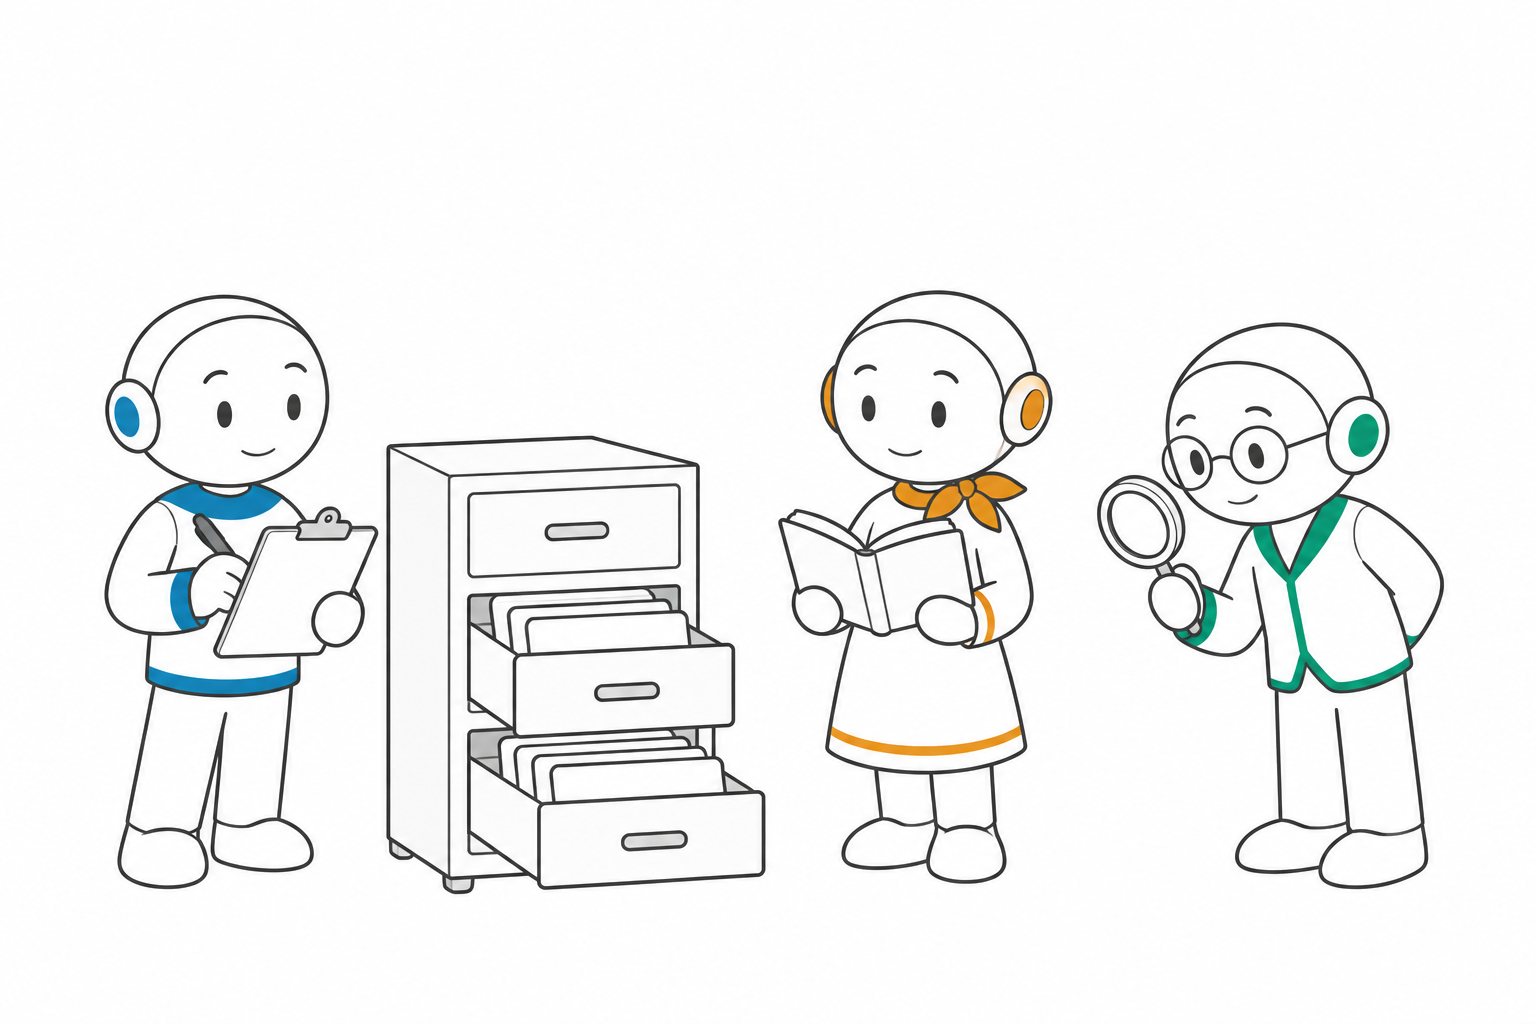
\includegraphics[width=0.46\linewidth]{../../assets/en/roles-memory-concept.png}\par
{\scriptsize 角色与记忆的概念插图，AI生成，不代表实验效果。}
\end{center}

\clearpage{\small\linespread{0.98}\selectfont\setlength{\parskip}{0pt}\tableofcontents}
\clearpage\pagenumbering{arabic}
\chapter{可执行约束下的数据合成与筛选}\label{ch:data}\section{研究目标与框架基础}
教学回答需要分别核对程序事实和任务完成情况。报对输出不等于解释了学生的误解，合理的讲解也可能给错变式答案。本章研究合成参考能否执行核验并追溯来源、筛选能否减弱表面偏好线索，以及仍有哪些局限。最终交付1000条监督微调（SFT）示范和500对偏好数据，不测量学生学习收益。

\subsection{NaturalThoughts：选择哪些推理示范}
NaturalThoughts包含推理生成与标注、样本选择、监督蒸馏三个环节~\cite{nat}。作者从NaturalReasoning抽取问题，以DeepSeek-R1产生推理轨迹和最终答案；领域、检查与回溯等策略、冗长程度等标注，用于区分多样推理和重复叙述。选择同时考察主题、语义或策略多样性，以及不同推理模型之间的答案分歧等难度代理。分歧不能证明任一答案正确。混合蒸馏为分歧题保留完整推理，其余题可仅保留最终回答，再监督学生模型。

证据具有规模条件：同一Llama-3.1-8B-Instruct在10万条样本下，分歧选择与随机选择的GPQA-Diamond正确率为45.2\%与42.5\%；50万条时则为45.2\%与48.3\%~\cite{nat}（第7页表1）。本项目借鉴分开记录选择属性、另外核验答案的思想，未复现DeepSeek-R1生成、论文标注或大模型蒸馏；结构难度也未按真实学生校准。

\subsection{Matrix：多阶段生产怎样执行}
Matrix将每条输入封装为可序列化的编排对象，保存流程状态、中间历史和路由决策~\cite{matrix}。队列驱动的角色逐步更新并转交对象，完成记录进入持久化输出；模型推理与容器工具由独立服务承担。逐条调度以及数据、任务、角色并行，让样本不必等待整批异质任务结束。系统监测队列、未完成任务和延迟；其至多执行一次语义意味着，角色重启不会自动恢复已出队的执行中样本，必须记录失败并按需离线重跑。

从网页合成推理数据时，文档筛选、题目与参考抽取、独立求解、按需核验是不同步骤。调度机制不决定答案质量，合格标准仍由任务检查给出。论文在相同模型、248张A100、各自并发设置下报告约为Coral的6.8倍吞吐，共识答案正确性指标接近~\cite{matrix}（第9页表1）。本地实现借鉴阶段分离和逐条溯源，没有部署分布式Matrix，也不据此宣称加速。

AIR区分偏好标注、指令选择与回答配对~\cite{air}；fDPO依据当前模型和奖励比较动态过滤~\cite{fdpo}；DEITA结合复杂度、质量和向量多样性~\cite{deita}。这些资料用于解释取舍，未照搬阈值或宣称获得论文中的模型增益。原始机制及结论边界见所引论文。

\begin{figure}[H]\centering
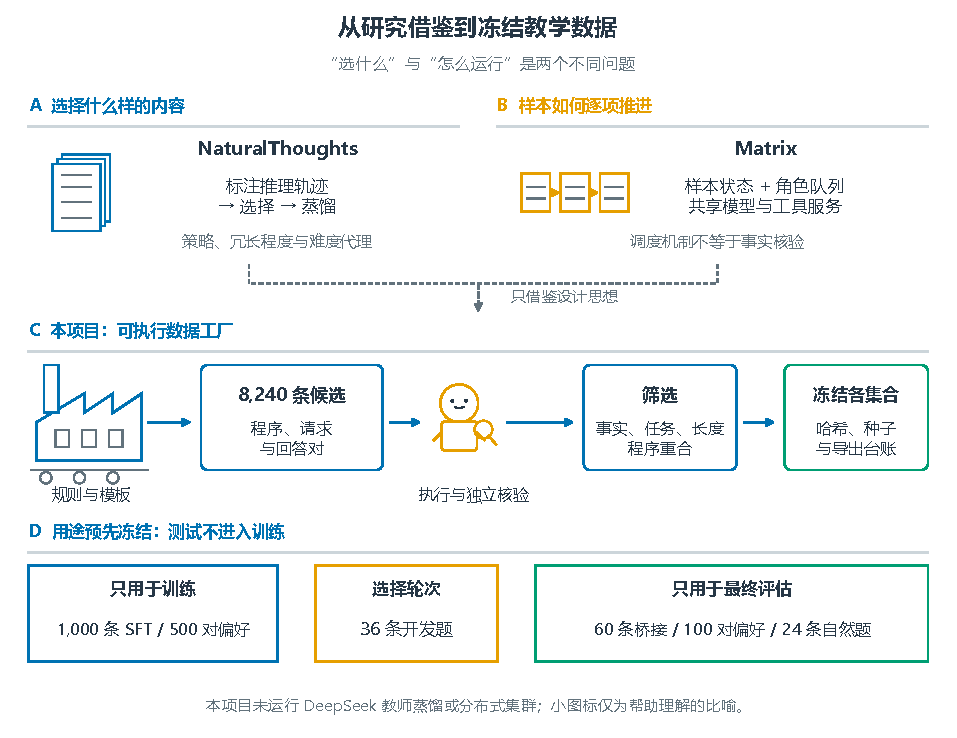
\includegraphics[width=\linewidth]{../../assets/zh/synthesis-atlas.pdf}
\caption{从两套研究框架的启发到可执行数据。框架机制、实际核验和冻结训练／评价导出分别标识。工厂与检验员是解释性比喻，不代表新增智能体或实验对象。}\label{fig:data-pipeline}
\end{figure}\FloatBarrier

\section{可执行数据构建与核验}
SFT记录包含用户与助教消息；偏好记录包含共同请求、首选和次选回答。元数据连接题族、任务、结构难度、种子、候选编号、程序、参考值、筛选去向和导出行号。修订生成器记录8240个候选，训练覆盖24个题族；预测、讲解、诊断、迁移各有250条SFT。500对偏好中，事实错误和指令不符各250对，后者例如遗漏明确要求的解释。这些是按规则构造的对比，并非自然采样的模型错误。冻结文件保持原始中文，没有逐条调用在线教师模型，也没有真实学生观察或教师偏好投票；英文版的例子是译文。

对原程序$P$及变式$P'$，独立计算的参考$y,y'$须满足
\begin{equation}
V(P,P')=\mathbf1\{\operatorname{stdout}(P)=y\}\mathbf1\{\operatorname{stdout}(P')=y'\}.
\label{eq:data-exec}
\end{equation}
独立核验脚本仅用标准库，不导入生成器或渲染器；检查明确标记的参考及负例类型，要求应改变答案的变式确实改变。跨集合核对规范化程序和请求，包括原题／变式的所有组合。另一粗粒度AST指标去除变量名与常量，用于暴露模板重复，与精确去重的目的不同；共同项目作者身份仍限制了独立性。

导出包括1000条SFT、500对训练偏好、三个留出题族的36条开发示范、逐字节保留的60条旧版桥接参考、100对偏好测试和24道另行编写的自然题。开发集选检查点，测试不参与。自然题由项目内Codex编写，部分主题与训练重合，检验新实例和问法，不代表全新知识。修订核验通过11234项异质检查，10个主要文件可逐字节再生；它支持可执行一致与溯源，不能解释为11234次教学评分通过。

\section{筛选对照与剩余捷径}
原版在同一1931对合格偏好候选上进行受控选择。50个共同排列比较随机选择A、任务／背景／缺陷均衡B、再加入长度优先C，各题族配额固定，每次均取500对；未打乱的C复现正式编号。50次只是同一候选池的顺序置换，并非独立采集。定义“总选长回答”的命中率
\begin{equation}
H=(n_{\mathrm{preferred\ longer}}+0.5n_{\mathrm{equal}})/N.
\label{eq:data-heuristic}
\end{equation}
标签偏差$D$为任务、背景、缺陷三轴上，族内频率与均匀分布总变差距离$\frac12\sum_k|p_k-1/K|$的配额加权均值。

\begin{table}[H]\centering\small
\caption{固定候选池的筛选：均值（50次置换样本标准差），$D$仅列均值。}\label{tab:data-ablation}
\begin{tabularx}{\linewidth}{@{}Yrrr@{}}\toprule
策略 & 首选较短（\%） & 选长命中$H$（\%） & $D$\\\midrule
A：随机 & 19.08（1.43） & 80.63（1.44） & 0.1112\\
B：标签均衡 & 19.39（1.03） & 80.31（1.02） & 0.0189\\
C：长度与标签 & 43.89（0.12） & 55.97（0.15） & 0.0278\\\bottomrule
\end{tabularx}
\end{table}\FloatBarrier

\begin{figure}[H]\centering
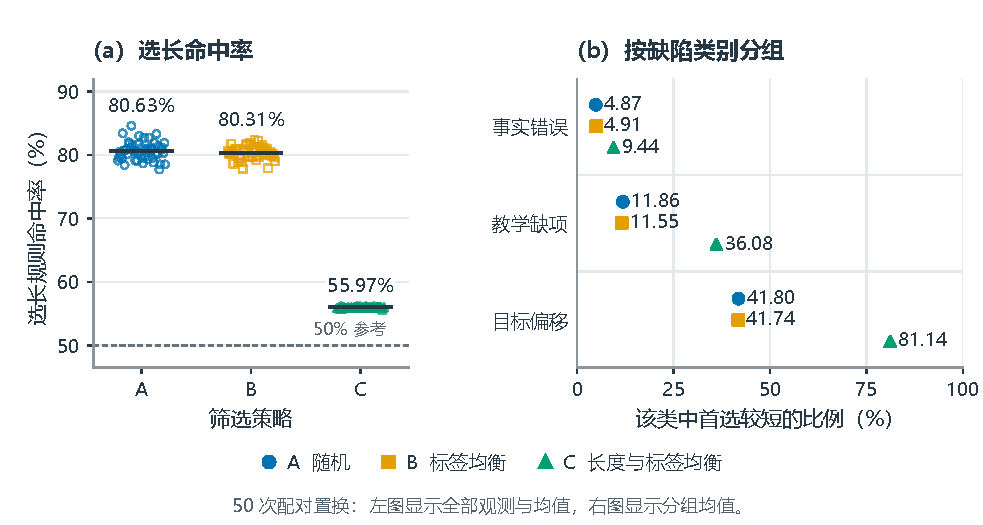
\includegraphics[width=\linewidth]{../../assets/zh/selection-ablation.pdf}
\caption{三种策略下实际可测的长度线索。散点保留50次配对置换，分类均值揭示总体均衡掩盖的差异。此对照没有训练模型。}\label{fig:data-ablation}
\end{figure}\FloatBarrier

C相对B在每次置换中均降低$H$：平均减少24.34个百分点，标准差1.02，范围为减少21.7至26.3个百分点；但$D$由0.0189升到0.0278，存在取舍。C的分类首选较短比例仍为事实错误9.44\%、教学缺项36.08\%、目标偏移81.14\%。

题族供给解释了为何不能按族各半得到250对较短首选：向下取整目标总计245，列表别名、循环控制、递归分别缺14、7、5对；七个奇数配额题族可各多取一对。因此各族尽量近半的总数范围是219--226，正式集220对，置换219--221对。整体取250对仅能通过部分题族补偿其他题族、偏离族内各半实现。

\begin{figure}[H]\centering
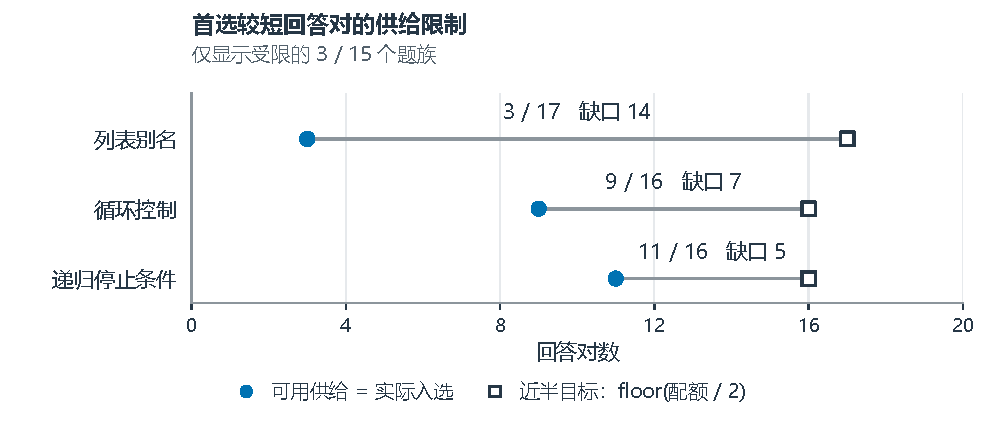
\includegraphics[width=\linewidth]{../../assets/zh/family-supply.pdf}
\caption{原15个训练题族中，三个题族的较短首选供给不足以达到配额一半的向下取整值；它们的全部可用较短首选均已入选，标注缺口给出约束来源。}\label{fig:data-family-supply}
\end{figure}\FloatBarrier

原版179条偏题次选还含互斥固定片段：58条有\verb|sep='-'|，62条有\verb|end=''|，59条有\verb|print('A#B')|；其余321条次选和500条首选均不匹配。修订删除这些已知线索并缩短回答，不能据此证明全部捷径消失。

\begin{table}[H]\centering\small
\caption{同口径正式发布集诊断。55.9\%是正式集结果，区别于55.97\%的置换均值。}\label{tab:data-revision}
\begin{tabularx}{\linewidth}{@{}Yrr@{}}\toprule
指标 & 原版 & 修订版\\\midrule
SFT／偏好AST结构数 & 105／98 & 145／121\\
SFT／首选字符中位数 & 306／296 & 65／64\\
选长回答命中率 & 55.9\% & 50.0\%\\
匹配已检固定片段的次选 & 179 & 0\\\bottomrule
\end{tabularx}
\end{table}\FloatBarrier

剩余耦合仍强：250条事实错误负例中，迁移122、诊断121、预测6、解释1；250条指令不符则全部来自预测／解释，偏好测试也有类似关联。1000条SFT均恰含一次固定输出标签，只对应145种结构和890种完整回答；36条开发示范仅四种结构。可执行并不等于教学与协议覆盖充分。

\section{结论与补充证据}
数据研究完成生成与筛选交付，并测量了特定表面线索的变化，没有证实推理改善、教师认可或学习收益。历史12例抽查属于非盲Codex检查，不能估计全库教学成功率。候选流量、不同指纹口径、逐条审阅及完整C00670偏好样本保留在数据与对照记录中。第二章实际检验更强的模型可靠性命题。

\begin{quote}\small\textbf{阅读注释。} 可以把SFT看作示范教材，把偏好对看作同题两种回答的比较。“首选”既可能因为算对，也可能因为更符合请求；不是越长越好。程序核验像检查答案的尺子，不能代替教师判断讲解是否有效。
\end{quote}
\FloatBarrier
\chapter{监督微调与偏好优化}\label{ch:training}\section{实验问题、模型与优化目标}
实验从官方\texttt{Qwen/Qwen2.5-0.5B}基础模型出发，使用筛选后的教育数据依次进行SFT和DPO。固定版本前缀为\texttt{e332bac62ed3}，权重、分词器和配置均有散列记录~\cite{qwenbase}。模型含494032768个参数、24个Transformer层，未用Instruct替代；第三章另行取得的Instruct诊断模型不算本项目训练成果。研究问题是：拟合示范和优化同题偏好，是否改善实际教学回答，以同题对照和事实复核检验。

LoRA冻结$W_0$，仅学习查询／取值投影的$(\alpha/r)BA$~\cite{lora}。共同ChatML序列化不添加系统轮次；完整回答包含结束标记，提示和补齐位置不计损失，入选训练样本没有静默截断。SFT最小化按回答token数归一化的负对数似然：
\begin{equation}
\mathcal L_{\mathrm{SFT}}=-\frac1T\sum_{t=1}^T\log\pi_\theta(y_t\mid x,y_{<t}).
\label{eq:training-sft}
\end{equation}
DPO的初始策略与冻结参考均来自所选SFT检查点，参考序列分数在更新前缓存。令$\ell_\pi$为完整回答的对数概率和，同题首选／次选为$y^+,y^-$：
\begin{align}
m_\theta&=\ell_{\pi_\theta}(y^+|x)-\ell_{\pi_\theta}(y^-|x)
-\bigl[\ell_{\pi_{\rm SFT}}(y^+|x)-\ell_{\pi_{\rm SFT}}(y^-|x)\bigr],\\
\mathcal L_{\mathrm{DPO}}&=-\log\sigma(0.1m_\theta).
\label{eq:training-dpo}
\end{align}
这一相对目标~\cite{dpo}不是事实正确率。初始策略与参考相同时，损失应为$\ln2$，与父检查点散列、实际参数变化一起构成训练链路核验。

\section{实际算力、训练与选模}
历史CPU实验使用i7-12700H、约16GB内存、六线程、float32；128条SFT和64对偏好各训练一次，末四层以$r=8$、$\alpha=16$适配，共90112个可训练参数，学习率分别为$8\times10^{-4}$和$2\times10^{-4}$。子集覆盖全部15个原训练题族，各用发布量的12.8\%，两个阶段均实际改变权重。后续同时改变数据与配置，故CPU结果单列，不混成同一受控比较。

\begin{table}[H]\centering\small
\caption{历史CPU结果：60题完整参考共13437个回答token；其余指标来自同一六题、贪心192-token上限。自动未判定不等于事实错误。}\label{tab:training-cpu}
\begin{tabularx}{\linewidth}{@{}Yrrrr@{}}\toprule
阶段 & 参考NLL & 自动对／错／未定 & 达到上限 & 四元重复（\%）\\\midrule
基础 & 3.276 & 0／0／6 & 6 & 44.9\\
SFT & 2.508 & 0／2／4 & 5 & 58.0\\
DPO & 2.664 & 0／0／6 & 6 & 72.8\\\bottomrule
\end{tabularx}
\end{table}\FloatBarrier

两次真实云端实验均将修订1000条SFT训练三轮、500对DPO训练一遍，另从同一所选父模型继续SFT更新500步。均用float32、批量1、$r=16$、$\alpha=32$、种子20261107及DPO系数0.1。继续SFT读取SFT集合，不是同一批DPO提示的首选侧；它匹配更新次数及部分配置，不匹配提示、token或严格算力。

\begin{table}[H]\centering\small
\caption{已记录的云端配置与开发集选择。耗时仅累计优化步骤，不含加载、参考缓存和评估。}\label{tab:training-protocol}
\begin{tabularx}{\linewidth}{@{}Yrr@{}}\toprule
设置 & 首次云端 & 探索性追加\\\midrule
适配Q/V层 & 末8层 & 全24层\\
可训练参数 & 360448 & 1081344\\
SFT学习率 & $2\times10^{-4}$ & $1\times10^{-4}$\\
DPO／对照学习率 & $1\times10^{-5}$ & $1\times10^{-5}$\\
SFT／DPO／对照步数 & 3000／500／500 & 3000／500／500\\
第1轮开发NLL & 2.6449 & 2.8672\\
第2轮开发NLL & 3.0709 & 3.3245\\
第3轮开发NLL & 3.3794 & 3.6293\\
SFT／DPO／对照步骤秒数 & 251.5／68.9／44.1 & 411.9／103.8／70.9\\\bottomrule
\end{tabularx}
\end{table}\FloatBarrier

每次运行分别处理143934个SFT回答token、48091个双侧DPO token和23981个对照token。36条开发示范的完整参考NLL在两版都选中第1轮、1000步，平局取较早轮次；3000步预算包含未入选轮次。开发集仅四种粗结构。追加方案在看过旧测试后制定，同时扩大适配层数、减半SFT学习率，属于探索性比较，不能单独归因。首次包独立记录CUDA，但未独立记录设备型号；追加两次尝试的Torch与\texttt{nvidia-smi}日志均记为T4，设备日志仍不是外部硬件认证。

\section{同题结果与全文复核}
固定评价包含24道Codex编写的自然题、100对未见偏好和60条逐字节保留的桥接参考。开发集不进入最终指标。各阶段提示一致，贪心生成上限384个新增token，保存全文、token及停止原因；NLL对含结束标记的完整参考按token加权。偏好胜出比例比较完整序列似然，受长度影响，不是人工偏好或学习收益。追加复用已见测试，未形成新的盲测。

独立分工的Codex代理阅读全文，保存散列、连续证据、主值解释和理由：唯一可辨且符合执行参考为对C；唯一可辨但不同为错W；缺答、复制输入、数值角色不明或多个未撤回的冲突断言为未判定U。解释事实另外核查。这是同项目非盲模型辅助审查，不是外部教师评分。

\begin{table}[H]\centering\small
\caption{云端配对结果：自然题24、桥接参考60、偏好测试100对。EOS只表示结束；对／错／未定来自完整主输出复核；偏好与重复列为百分比。}\label{tab:training-cloud}
\begin{tabularx}{\linewidth}{@{}Yrrccrr@{}}\toprule
阶段 & 自然NLL & 桥接NLL & EOS/24 & 对／错／未定 & 偏好 & 重复\\\midrule
基础 & 3.7258 & 3.2758 & 7 & 3/3/18 & 43 & 63.3\\
首次SFT & 3.5892 & 4.0081 & 1 & 1/20/3 & 47 & 79.2\\
首次DPO & 4.2992 & 4.5216 & 1 & 0/7/17 & 51 & 76.3\\
首次对照 & 3.4445 & 3.9352 & 0 & 1/19/4 & 47 & 82.5\\
追加SFT & 3.5873 & 4.2234 & 8 & 3/16/5 & 45 & 55.7\\
追加DPO & 6.6152 & 6.7619 & 11 & 4/7/13 & 53 & 31.2\\
追加对照 & 3.5764 & 4.3570 & 7 & 5/11/8 & 47 & 63.0\\\bottomrule
\end{tabularx}
\end{table}\FloatBarrier

首次DPO相对SFT使24道自然题与60条桥接参考的NLL全部升高；继续SFT使84条全部降低，却仍未交付可靠教学。追加SFT减少重复、增加结束，但自然NLL相对首次仅变化$-0.0019$。追加DPO再次使84条参考全部变差，同时偏好胜出45\%升到53\%、EOS由8升到11。不同端点不支持一个笼统的“效果改善”结论。

\begin{figure}[H]\centering
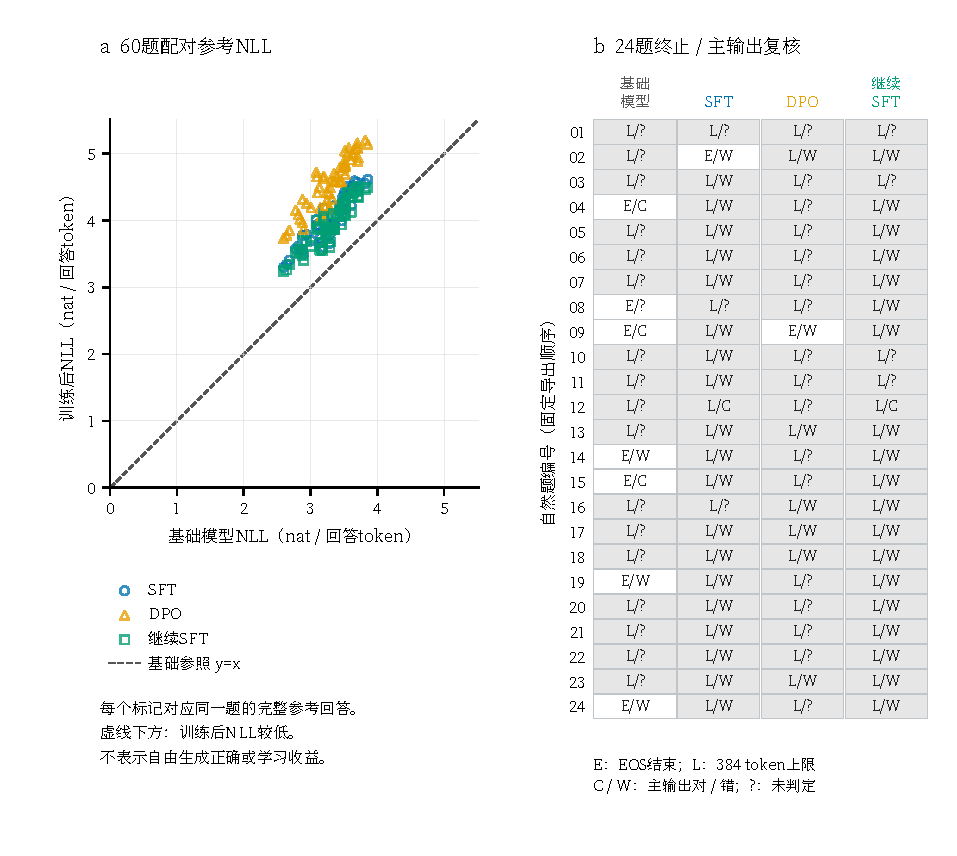
\includegraphics[width=\linewidth]{../../assets/zh/training-v2-evidence.pdf}
\caption{首次云端逐题证据：每阶段60条桥接配对NLL，以及24条自然题的终止／输出记录。E为EOS，L为384-token上限，C/W/?仅为全文主值判断，解释另评。所有点均为已记录观测，不作跨种子显著性声明。}\label{fig:training-v2-evidence}
\end{figure}\FloatBarrier

追加SFT的三个正确主值均伴随解释错误；追加DPO四个正确主值中，三个解释错、一个不明；追加对照五个正确主值中，三个解释错、一个不明，一个未发现直接错误但仍严重重复。例如SFT对\verb|137 // 12|答11却称无余数，实际余5；对\verb|[173,179,181,191][-2]|答181却称负下标从0开始。主值正确不能算完整教学成功。追加24条基础输出与首次逐字相同，经核验复用旧评分；72条新增训练后回答均重新阅读全文。

\begin{figure}[H]\centering
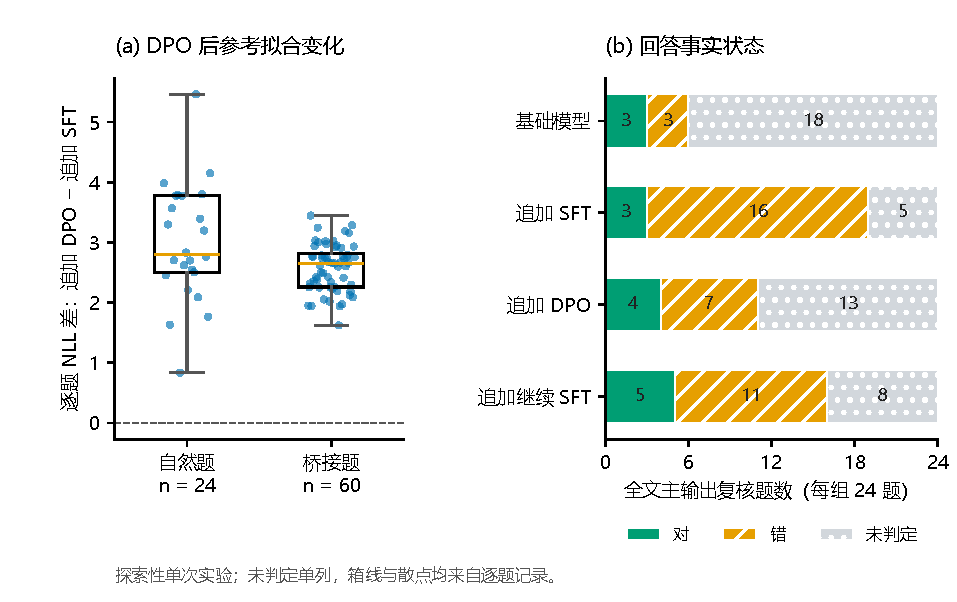
\includegraphics[width=\linewidth]{../../assets/zh/training-retry-comparison.pdf}
\caption{追加DPO相对SFT的参考NLL及主输出复核。24条自然题、60条桥接题的NLL全部变差；箱体概括实际逐题分布，不表示多训练种子不确定性。未判定与错误分开保留。}\label{fig:training-retry-comparison}
\end{figure}\FloatBarrier

\section{两道固定题：任务、执行参考与实际回答}
以下固定取自然测试导出顺序前两题，没有按成功挑选。片段来自原始中文实录，仅合并排版空白、去除代码反引号，省略号标记删节；表中判断依据完整回答，包括短片段之外的冲突，未修改原评分规则。英文版逐项翻译，不是新生成英语回答。

\Needspace{25\baselineskip}
\subsection{NATURAL-01：赋值保存先前值}
\begin{quote}\small
我以为saved会跟着wallet一起变小。你能告诉我实际打印什么，并解释这种理解哪里不对吗？
\begin{verbatim}
wallet = 137
saved = wallet
wallet = wallet - 18
print(saved)
\end{verbatim}
\end{quote}
执行参考为\texttt{137}：重新绑定\texttt{wallet}不会改变\texttt{saved}已经绑定的整数。

\begin{table}[H]\centering\small
\caption{固定案例01：短实录与完整回答主值判断。}\label{tab:training-case01}
\begin{tabularx}{\linewidth}{@{}lYc@{}}\toprule
阶段 & 实际回答摘录 & C/W/U\\\midrule
基础 & “将wallet的值减去18并将结果存储在saved变量中”；完整回答无唯一原题主值。 & U\\
首次SFT & “本题输出：49”……“本题输出：101”。 & U\\
首次DPO & “本题输出：79”……“本题输出：80”。 & U\\
首次对照 & “本题输出：119”……“print出来的结果是117”。 & U\\
追加SFT & “本题输出：119”；“print(saved)的输出是119”。 & W\\
追加DPO & “本题输出119”……“本题输出：18”。 & U\\
追加对照 & “本题输出：119”；“把wallet作为参数传递给-18，变成了[137]”。 & W\\\bottomrule
\end{tabularx}
\end{table}\FloatBarrier

错误涉及赋值语义，不只是漏写输出标签。重复或竞争数值不能靠挑选一个方便的数字解决，也不能把从题面复制的137计为独立算对。

\Needspace{25\baselineskip}
\subsection{NATURAL-02：拆分、切片与拼接}
\begin{quote}\small
我在处理树木标签。这里只截了哪些名字？最后连起来的文本是什么？请直接用这个例子解释。
\begin{verbatim}
label = 'oak|pine|elm|ash'
parts = label.split('|')
print('/'.join(parts[1:3]))
\end{verbatim}
\end{quote}
执行参考为\texttt{pine/elm}：选下标1、2，连接符为斜杠。

\begin{table}[H]\centering\small
\caption{固定案例02：代码与输出字符串保持原拼写。}\label{tab:training-case02}
\begin{tabularx}{\linewidth}{@{}lYc@{}}\toprule
阶段 & 实际回答摘录 & C/W/U\\\midrule
基础 & 重复完整问题和代码后接“erable”，没有断言结果。 & U\\
首次SFT & “本题输出：/oak|pine|elm|ash”；称切片保留oak和pine。 & W\\
首次DPO & “本题输出：/amel|ash|elm|ash”……重复\texttt{|ash}。 & W\\
首次对照 & “本题输出：/oak|pine|elm|ash”。 & W\\
追加SFT & “本题输出：oak|elm”；“只保留第1和第3个部件”。 & W\\
追加DPO & “本题输出：oak|elm”……“本题输出：['oak', 'oak', 'elm', 'elm', 'elm']”。 & U\\
追加对照 & “本题输出：oak|elm”；“把第1个和第3个分号去掉”。 & W\\\bottomrule
\end{tabularx}
\end{table}\FloatBarrier

原程序、完整请求、七阶段回答、停止原因和逐题审阅，仍在\path{training/retry_imports/retry_048f9a92c0ef_numeric_review/comparison/}及关联JSON中；短片段不替代或暗删失败证据。

\section{审计异常、退化分析与停止决定}
首次云端导入通过552项一致性检查；追加初次965项检查中，一项首步策略／参考阈值失败。次选序列分数相差$1.52587890625\times10^{-5}$，是该量级float32的一个相邻可表示间距，大于旧绝对阈值$10^{-5}$；损失与$\ln2$相差$7.77\times10^{-7}$。原失败审计保留。事后结构化复审允许每序列至多一个间距，同时检查比值、相对边际、DPO缩放／损失运算与冻结缓存完全一致；966项均通过，边界测试仍拒绝更大或不一致差异。CPU探针没有复现T4归约的具体原因；复审未改权重、回答或事实标签，只证明范围内内部一致，不能证明教学有效。

检查未发现明显的提示损失掩码反向、因果位移、漏结束符或截断丢结束符。开发NLL在第1轮后持续上升；DPO只保存500步终点，没有中间开发退出，不能事后宣称早停。追加第401--500步的100组更新前训练对快照中，96组两侧分数均低于冻结SFT参考；策略减参考的均值为$-37.761/-59.936$ nat，首次对应84组、$-8.550/-13.065$。每组使用当步训练对，并非一次更新前后之差或终点固定集曲线。记录显示相对偏好间隔增大可与绝对似然较低并存，尚不能单独确认生成退化的原因；

\paragraph{已观察的限制与可能原因。} 1000条SFT样本只有145种粗粒度程序结构；偏好负例理由与任务类型存在关联，36条开发集仅覆盖四种结构。第一轮后开发NLL变差，追加实验中24条自然题的参考NLL从SFT的3.5873升至DPO的6.6152。这些是覆盖有限和参考拟合退化的证据，不能单独证明原因。

小基座模型的能力、模板狭窄、偏好数据中的表面线索以及训练设置都可能有影响。本项目未在相同协议下比较更大基座；追加实验同时改变适配层范围与学习率，继续SFT对照的提示和token预算也不同。因此无法量化模型规模或某一设计的因果贡献；过拟合仍是推测。本次未新增训练或模型推理。

\begin{figure}[H]\centering
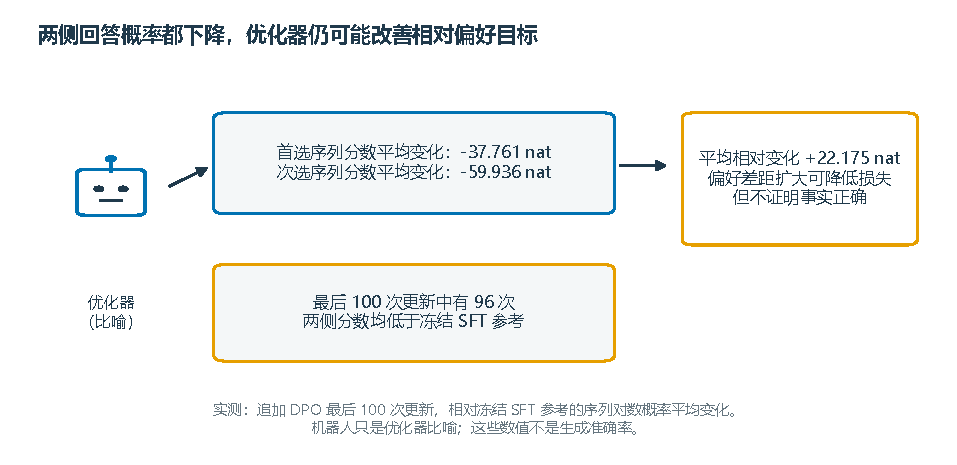
\includegraphics[width=\linewidth]{../../assets/zh/training-objective-gap.pdf}
\caption{两侧回答概率都下降，相对偏好目标仍可能变好。数值是第401--500步更新前当步训练对相对冻结SFT的分数，并非各次更新造成的变化；机器人只是比喻，序列对数概率不是正确率或学习收益。}\label{fig:training-objective-gap}
\end{figure}\FloatBarrier

仅做一次调用前固定方案的本地有限补救：混合有效适配更新，而不分别插值低秩矩阵因子：
\begin{equation}
\Delta W_\lambda=(1-\lambda)\Delta W_{\mathrm{SFT}}+\lambda\Delta W_{\mathrm{DPO}}.
\end{equation}
没有优化器更新，全部36条开发参考选择固定候选；差异小于$10^{-6}$时保留较小系数。

\begin{table}[H]\centering\small
\caption{开发集有限混合。0为SFT父模型，1为完整DPO；属于事后校准，不是新盲测训练成果。}\label{tab:training-remedy}
\begin{tabular}{@{}lrrrrr@{}}\toprule
$\lambda$ & 0 & 0.05 & 0.10 & 0.25 & 1\\
开发NLL & 2.8672 & 2.9447 & 3.0290 & 3.3237 & 5.9292\\\bottomrule
\end{tabular}
\end{table}\FloatBarrier

最终选0，仅支持在此候选族中收回DPO改动，没有修好SFT。六条预定开发题继续比较重复惩罚1.0／1.08，均为贪心192-token上限：EOS由1/6到3/6，生成970降到717 token；两组仍各为对0、错4、未判定2。字符串\texttt{aabbbbbab}有六个\texttt{b}，两组均报三；参考112的循环分别报125、248，布尔竞争断言继续未判定。开发集复用且只有四种结构，不是独立验证。

明确事实错误触发预登记停止条件；后续未继续优化，未继续云端训练、测试集调参或新增部署。扩展数据、交叉均衡偏好理由、中间检查点和监督锚定仍属未执行方案。完整回答、逐步日志、数值审计与有限补救记录保留在\path{training/}。本项目完成可运行的SFT--DPO链路，但教学可靠性较差，没有把失败改写成成功。

\begin{quote}\small\textbf{阅读注释。} NLL低表示参考文字更容易被模型预测，不是答题正确率；EOS只表示回答结束。DPO比较两份回答的相对变化，所以两边概率都降低也可能得到更低损失。读表时应把主值、解释、终止和学习收益分开；“未判定”也不能直接算错。
\end{quote}
\FloatBarrier
\chapter{可核验的教学智能体与学习者记忆}\label{ch:agents}\section{研究问题与 OpenMAIC 机制}
本章检验角色分工、可执行证据和持久学习记录，能否把能力有限的教育语言模型组织成可核验的教学流程。评价区分完整系统与模型本身：成功检索历史或给出正确回退答案，不等于模型已经能够自主教学。研究问题分别涉及调度机制、跨轮学生证据，以及教学请求成功或失败的具体原因。

源码分析固定于 OpenMAIC 官方提交 \texttt{5bd8cc840ee63}，检索日期为2026年11月6日\cite{openmaic}。完整提交号、永久链接与19份归档文件的 SHA-256 见 \path{tutor/legacy/research/source_manifest.json}。本项目没有部署原 OpenMAIC；后续 Python 系统是独立简化实现，主要借鉴表\ref{tab:concise-agents-source}中的四类机制。

\begin{table}[htbp]\centering\small
\caption{OpenMAIC 的实际机制与固定源码锚点。表内路径相对固定的上游仓库，永久链接保留于来源清单。}\label{tab:concise-agents-source}
\begin{tabularx}{\linewidth}{@{}p{25mm}Yp{65mm}@{}}\toprule
机制 & 源码实际实现 & 来源位置\\\midrule
角色与调度 & 教师、助教、同学具有不同提示和动作；Director 用 \texttt{call\_agent} 选择有用的发言者，并非固定轮流。子角色可共享模型对象；结束动作检查是否已有可见回应或实质教学内容。 & \path{registry/built-in.ts}:12--155；\path{pi/director-loop.ts}:95--221；\path{pi/tools/call-agent.ts}:735--757、847--864。\\
课程状态与证据 & 材料分析、资料研究先于大纲和场景生成；完成步骤是显式状态。\texttt{read\_scene} 向后续角色提供页面证据，限制无依据猜测。 & \path{generation/run/plan.ts}:45--103；\path{generation/src/scene-builder.ts}:21--116；\path{pi/tools/read-scene.ts}:97--124。\\
上下文与记忆 & 子角色保留最近12条消息；Director 压缩时保留目标与未解决问题。PBL Instructor 在历史超过30条后向最近16条压缩，提取学习线索并读回 \texttt{earlierSummary}；摘要压缩阈值为4500字符。 & \path{pi/prompts.ts}:558--589；\path{pi/director-compaction.ts}:95--101、136--217；\path{v2/agents/instructor-memory.ts}:22--138。\\
反馈与回退 & 测验区分提交前后状态，提交后的学生答案、参考、评分和评语用于反馈。模型评分无法解析时可回退半分；这维持接口运行，并不能证明答案正确。 & \path{summarizers/state-context.ts}:172--240；\path{api/quiz-grade/route.ts}:56--105。\\\bottomrule
\end{tabularx}
\end{table}\FloatBarrier

因此，OpenMAIC 不只有聊天历史，还包含场景状态与显式学习者摘要；但由关键词提取的进度线索不等于经过核验的掌握度。本项目保留分工、共享证据和显式控制，将多媒体课堂缩小为可执行的 Python 输出题，不复现语音、白板和完整课程编辑器。

\section{实现与可核验学生记忆}
控制器顺序调用规划、教学、评审角色，三者共享一次加载的模型。原版使用第二章 SFT；后续分别接入真实云端 SFT 检查点和明确区分的官方 Instruct 模型，本章不更新权重。规划返回关注点和策略；教学返回答案、反馈、解释及可选 \texttt{followup\_code}；评审返回 \texttt{approved} 和理由。实际提示为中文；完整模板、逐次上下文、原始回应、token 编号、停止原因和采用决定均留档。

受限 AST 解释器计算输出与轨迹，不把生成文本交给无限制的 \texttt{eval}/\texttt{exec}。评估器另用 CPython 执行已审阅、冻结的参考程序；不支持的程序不能直接取得参考答案并冒充已核验。原版采用门槛检查答案、必需解释/反馈文本、评审批准及复测可执行性；修订控制器才增加学生状态、事实证据和明确变式修改约束，历史C08运行尚无这些较强检查。这不能证明全部自然语言解释。被拒草稿保留，最终回答明确标注工具或模板回退来源。

原版在本机 CPU 上以 float32、六线程和贪心解码运行，每角色最多生成256个新 token；输入与生成合计超过4096时明确报错，不静默截断。修订角色预算为64/192/96。各组分别冻结实现、模型、提示和预算。

\begin{figure}[htbp]\centering
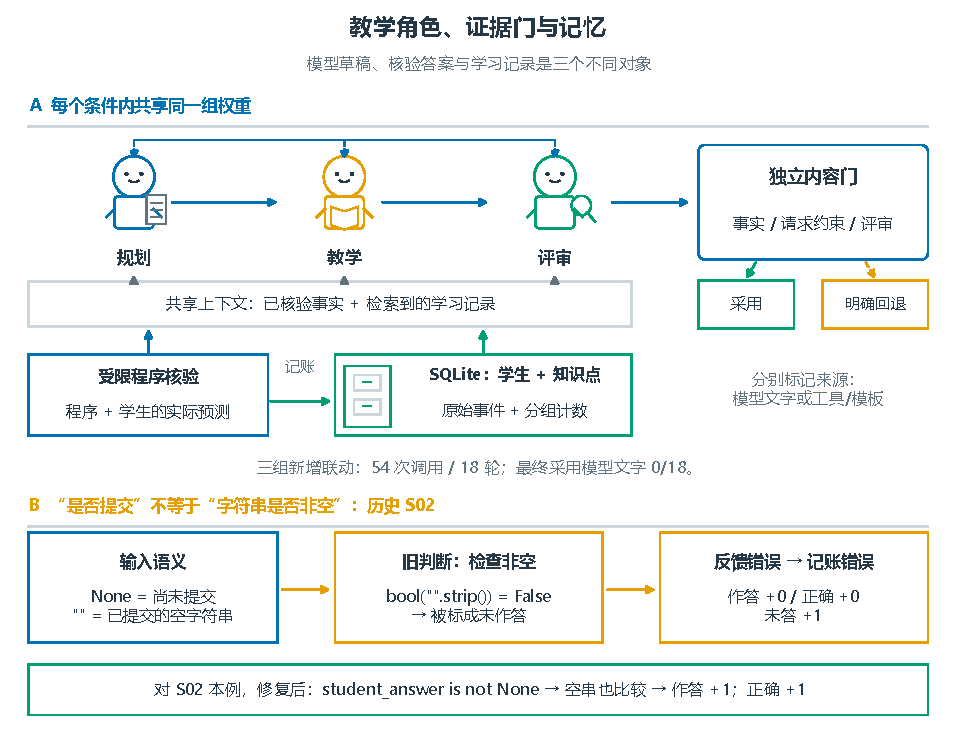
\includegraphics[width=\linewidth]{../../assets/zh/teaching-memory.pdf}
\caption{共享模型、角色调用、独立核验与学生记忆。历史空字符串故障与后续修复分开标记；角色形象只解释职责，不代表独立训练的模型。}\label{fig:concise-agents-system}
\end{figure}\FloatBarrier

SQLite 保存原始事件和派生统计。事件包括学生标识、主题、程序、预测、证据、角色输出及最终回答；统计区分交互、作答、正确、错误、未答和未核验。两层在同一事务中写入，重复事件编号不能再次计数；模型答案不算学生作答。对学生 $u$、主题 $k$、结构难度 $d$，令 $v_t$ 表示执行已核验，$a_t$ 表示已提交预测，$z_t$ 表示预测与核验输出一致，则
\begin{equation}
N_{u,k,d}\leftarrow N_{u,k,d}+v_ta_t,\qquad
C_{u,k,d}\leftarrow C_{u,k,d}+v_ta_tz_t.
\end{equation}
这些是描述统计，不是校准后的掌握概率。原版以非空文本近似 $a_t$，其问题由 S02 实测揭示。

检索按调用者提供的学生ID与主题匹配，读入最近三条事件；这以可信调用者为前提，ID过滤不等于身份认证。重建系统对象后仍读取同一数据库。难度建议从最近100条相关事件中提取同一结构难度的可核验预测，并纳入本轮：连续三次正确建议升级，连续两次错误建议降级，其余保持；实际交付题目是否更难另行检查。显式主题键、受限语法和未校准阈值限制了个性化，尚未实现同义词、前置知识依赖和遗忘推理。

\section{历史协议与四个完整案例}
原批次在运行前冻结8个场景、11轮；观察后再冻结追加4个场景、6轮。参考包含原批22段、追加12段程序及变式，均独立执行。完整成功要求全部必要自动检查与全部预设定性条目通过。Codex 技术审阅保留原文依据，不属于教师盲评。追加设计者未读实现，但已看原案例与结果，因而属于定向覆盖扩展，不是随机样本或全程外部盲测。

两批共12个场景，7项完整、5项未完整，自动检查145/150；51次真实角色调用均未采用，17轮最终回答全部来自工具和模板。C03/C04 超过各自事前“部分完成”预期；C08/S02 低于各自运行前“完整完成”预期。C07 始终是预期内限制，没有为了凑数改标。C03 冻结理由曾提及此前“range/配对误答”，但 训练研究 未实际测试 range 生成；该措辞仅保留为跨概念风险推测，不作为已观察的先前 range 故障。

\begin{figure}[htbp]\centering
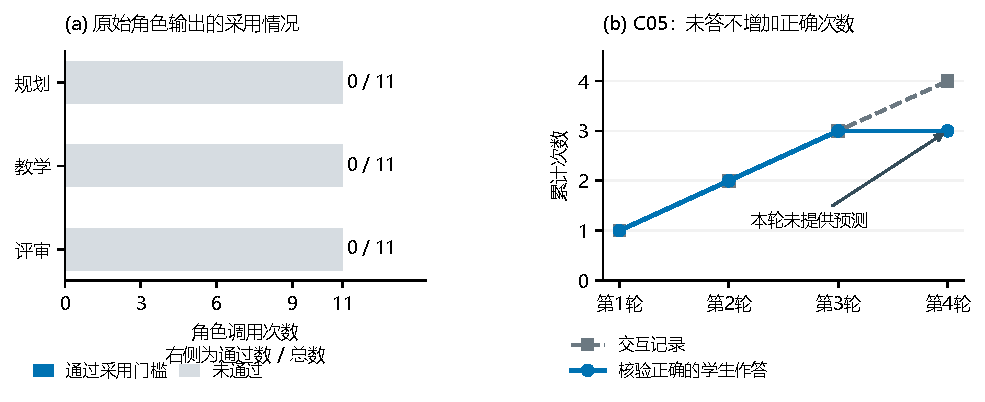
\includegraphics[width=\linewidth]{../../assets/zh/agents-evidence.pdf}
\caption{历史观测：原批11轮中角色输出采用均为零；C05 第四次交互未提交预测，因此正确作答数保持为3。自动记账与教学任务完整性是不同指标。}\label{fig:concise-agents-evidence}
\end{figure}\FloatBarrier

以下保留实际中文回答摘录。完整题目、参考、角色原文、最终回答及散列见 \path{tutor/legacy/results/core/}、\path{tutor/legacy/results/supplement/}；四案例的原文与英文完整译文还见 \path{reports/case-study-evidence.en.json}。

\Needspace{18\baselineskip}
\subsection{C03：跨实例取回旧错因}
\paragraph{任务与参考。}
学生此前把 \texttt{range(2,8,2)} 的终点8计入，预测20而非12。本轮重建系统对象后，预测下列程序为9，要求联系旧错误反馈，并提供给定的同概念复测：
\begin{verbatim}
total = 0
for n in range(3, 9, 3):
    total += n
print(total)
\end{verbatim}
正确结果为 $3+6=9$，终点9排除；给定复测将终点改为12，得到 $3+6+9=18$。

\Needspace{15\baselineskip}
\paragraph{实际回答与解释。}
原始教师反复生成核对错因的指示，未形成合格结构化回答，被拒绝。最终回答摘录为：
\begin{quote}\small
上次同一概念的记录中，你的预测与实际输出不一致。你写的预测是 '20'，核验输出为 '12'。当时你的原话是「我把 8 也加进去了，所以猜 20」。这只是作答证据，不等于掌握结论。

本题输出：9

你的这次预测与程序实际输出一致。

第 2 行（主程序）：range(3, 9, 3) 实际取值 [3, 6]；终点 9 不包含在内。

复测参考输出：18
\end{quote}
数据库保留两次预测、一对一错。检索跨对象重建仍有效，并保留旧证据，超过事前部分完成预期；引用来自确定性数据库读取，解释来自执行轨迹，不是已证明的模型学习者推理。

\Needspace{17\baselineskip}
\subsection{C04：同主题下隔离新学生}
\paragraph{任务与参考。}
另一名学生没有提交预测，请求解释下列程序并交付给定复测，不能继承上一名学生的经历：
\begin{verbatim}
total = 0
for n in range(2, 8, 2):
    total += n
print(total)
\end{verbatim}
原题为 $2+4+6=12$；给定复测将终点改为10，得到 $2+4+6+8=20$。作答数和正确数均应保持零。

\Needspace{13\baselineskip}
\paragraph{实际回答与解释。}
原始教师反复列出提取执行步骤、生成复测片段的指示，没有可用回答。最终工具和模板反馈为：
\begin{quote}\small
本题输出：12

这次未提供预测，因此不记录为作答正确或错误。

第 2 行（主程序）：range(2, 8, 2) 实际取值 [2, 4, 6]；终点 8 不包含在内。

复测参考输出：20
\end{quote}
检索结果为空，写入后该学生交互1次、作答0次、未答1次；没有引用旧学生错因，超过部分完成预期。这验证本次身份隔离，不证明系统能深度适应不同学习背景。

\Needspace{21\baselineskip}
\subsection{C08：执行正确，但变式违反修改约束}
\paragraph{任务与参考。}
学生预测230，要求列出各对贡献、未配对尾项，并且\emph{只在右列表末尾追加一个数}形成复测。原题与实际交付代码并列如下：
\par\noindent\begin{minipage}[t]{0.48\linewidth}\small
\textbf{原题程序}\par
\begin{verbatim}
left = [9,24,17,32,6,18]
right = [7,16,35,22,44]
total = 0
for a, b in zip(left, right):
    total += a + b
print(total)
\end{verbatim}
\end{minipage}\hfill
\begin{minipage}[t]{0.48\linewidth}\small
\textbf{实际交付复测}\par
\begin{verbatim}
left = [9,24,17,32,6,18]
right = [7,16,35,22,44]
total = 1
for a, b in zip(left, right):
    total += a + b
print(total)
\end{verbatim}
\end{minipage}\par
五对贡献为 $16,40,52,54,50$，合计212；左侧末尾18无配对。参考在右侧追加6，得到 $212+18+6=236$；其他追加值也可合法，只需代码和解释一致。

\Needspace{8\baselineskip}
\paragraph{实际回答与根因。}
不合格的原始教师回应被拒。最终回答正确给出212及逐对贡献，却又交付：
\begin{quote}\small
复测题：只把原第 3 行的 0 改为 1，其余不变。

复测参考输出：213
\end{quote}
代码确实输出213，但改的是累加初值，右列表未增长，仍只有五对。原有5项自动检查全部通过；缺失的是修改是否符合教学请求，而不是能否运行。该案例低于事前完整完成预期，是原批真正的意外失败。

\Needspace{20\baselineskip}
\subsection{S02：正确空字符串预测被当作未答}
\paragraph{任务与参考。}
学生显式提交 \texttt{student\_answer=""}，原话为“我的预测是空字符串，也就是只打印一个空行”。原题与给定复测为：
\begin{verbatim}
word = 'python'
print(word[4:1])   # Original
word = 'python'
print(word[1:4])   # Supplied follow-up
\end{verbatim}
默认正步长使 \texttt{[4:1]} 选不到下标。CPython 原始输出恰为一个换行，归一化后为空字符串，与预测一致；作答和正确应各加1，未答不变。复测参考为 \texttt{yth}。

\Needspace{12\baselineskip}
\paragraph{实际回答与根因。}
原始教师误称原切片返回 \texttt{python}，被拒绝。最终回答的输出字段确实为空：
\begin{quote}\small
本题输出：

这次未提供预测，因此不记录为作答正确或错误。

第 2 行（主程序）：word[4:1] 取下标 []，得到 \texttt{''}。

复测参考输出：yth
\end{quote}
不能在第一行冒号后补写系统未曾说出的“空字符串”。执行与复测正确，反馈和 SQLite 却将显式预测标为 \texttt{unanswered}：作答与正确保持零、未答增加1，自动检查仅5/9。\texttt{bool(student\_answer.strip())} 在比较答案前将有效空内容合并为未提交。这是不同于 C08 的状态表示故障，低于追加批运行前的完整完成预期，补齐第二个真正意外失败，无需更改 C07 标签。

\begin{figure}[htbp]\centering
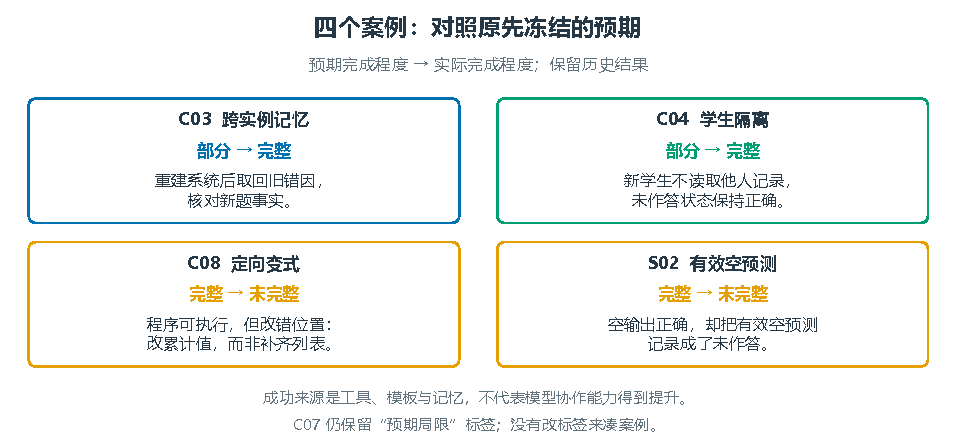
\includegraphics[width=\linewidth]{../../assets/zh/case-outcomes.pdf}
\caption{四个历史案例与各自运行前预期。C03/C04 成功依赖已核验记录和模板；C08/S02 暴露不同控制器缺陷。后续修复不抹去原结果，也不将历史失败改成新成功。}\label{fig:concise-agents-cases}
\end{figure}\FloatBarrier

\section{修复、对照与模型联动}
修复隔离在 \path{tutor/core/}，原输入、数据库、文件、预期和标签保持不变；已知案例回归不算未知测试。14项单元测试另覆盖否定、修改范围、空白输出、错误状态和身份隔离，脚本后端仅用于单元测试。

C07 的漏练习来自12字符窗口遇到16字符间隔。修订识别器去掉窗口并检查否定；受限的空列表、空字典默认值修复使用 \texttt{None} 和入口新建容器。C08 要求删去右列表新增元素后恢复原 AST，追加1输出231，是参考236之外的合法变式。S02 区分 \texttt{None} 与已提交空文本，规范化仅删末尾一次换行；修复计数为作答+1、正确+1、未答+0。首版修复工具卡把默认表达式列表 \texttt{[None]} 误当作可变默认容器，而函数实际默认参数已是 \texttt{None}；后来统一管线按类型和入口 AST 纠正。代码正确未自动保证说明正确。

\begin{table}[htbp]\centering\small
\caption{控制器与记忆对照。采用模型文字不等于教学质量达标。}\label{tab:concise-agents-controls}
\begin{tabularx}{\linewidth}{@{}Yrrrr@{}}\toprule
配置 & 轮数 & 调用 & 最终采用 & 检查\\\midrule
工具模板，开启记忆 &17&0&0&209/209\\
同系统，关闭记忆读取 &17&0&0&204/209\\
官方 Instruct，多角色 &17&51&1&209/209\\
官方 Instruct，单角色子集 &6&6&1&70/70\\\bottomrule
\end{tabularx}
\end{table}\FloatBarrier

关闭记忆仍写审计事件，但少了 C03/S03/S04 三次历史检索，以及 C05 难度建议、交付两项检查，支持这些机制在本次输入中的作用，不证明模型记忆推理或学习收益。官方 Instruct 是外部诊断，不代替自训练 SFT。17份教师原文中13份复制数值示例；17份评审全部批准，包括错误草稿。仅 C03 通过外部门槛，其采用文字逐字复述 F1 工具卡。同六题的单、多角色教师原文与最终文本相同，调用6对18次、生成耗时约35.0对73.5秒，没有观察到最终回答增益。

\begin{table}[htbp]\centering\small
\caption{相同八个新挑战上的提示与证据诊断。任务在调用前冻结但受已见故障启发；围栏兼容看过同题输出后修订，属于探索性复测。}\label{tab:concise-agents-prompt}
\begin{tabularx}{\linewidth}{@{}Yrrrr@{}}\toprule
条件 & 调用 & 教师解析 & 最终采用 & 检查\\\midrule
去示例，自由解释 &24&8/8&1/8&64/64\\
去示例，裸 JSON 严格引文 &24&0/8&0/8&64/64\\
完整围栏兼容复测 &24&8/8&1/8引文&64/64\\\bottomrule
\end{tabularx}
\end{table}\FloatBarrier

自由解释答案匹配7/8，学生状态仅2/8，唯一采用只是通用工具说明。严格组围栏内字段人工核读为答案7/8、状态3/8，但正式裸 JSON 解析仍为零。完整围栏兼容恢复结构读取，却没有修好这些状态；7次评审批准仍违反内容合约。只有 P03 采用\emph{模型选择的工具证据}，不是独立自由解释。教师原文与前严格组相同，解析使评审输入改变，因此是真实管线重跑，不能把离线解析算作新模型推理。原六题的探索性配对每条件18次调用：自由解释采用2/6，但一例从一次正确预测过度推断理解；严格引文解析和采用均为零。两组70/70来自核验与回退。提示、控制器和工具卡同时改变，不能视为纯提示消融。

\begin{figure}[htbp]\centering
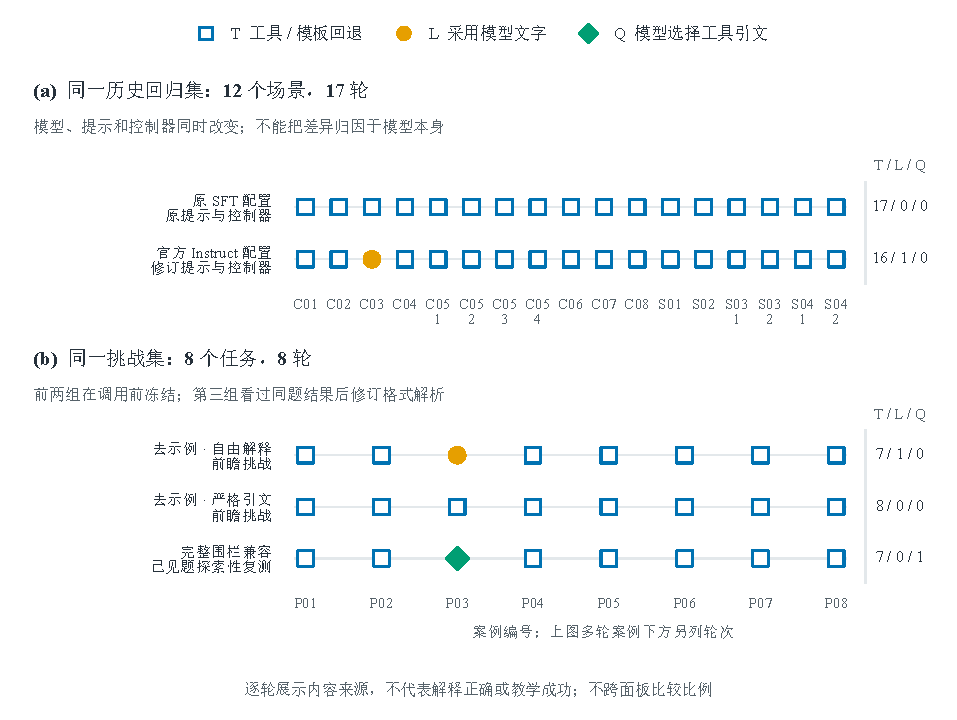
\includegraphics[width=\linewidth]{../../assets/zh/agents-revision-provenance.pdf}
\caption{实际记录的最终内容来源：工具模板、采用模型原文和模型选择工具引文。两面板任务集不同，不比较总体采用率；选择引文不证明独立推理或教学价值。}\label{fig:concise-agents-provenance}
\end{figure}\FloatBarrier

真实云端检查点另行联动：首轮 SFT 来自 首次云端运行，追加 SFT 来自 探索性追加运行。各组使用相同已知六题、64/192/96预算、本机 CPU float32 和贪心解码，未加载 DPO。Instruct 官方封装比 SFT 多21个系统开头 token；历史事件编号、规划采用和草稿也可能改变后续上下文，不能作只替换权重的因果比较。

\begin{table}[htbp]\centering\small
\caption{相同六题的四组自训练 SFT 部署。每组18次真实调用、工程检查70/70；正常结束只表示结束标记，不表示回答正确。}\label{tab:concise-agents-sft}
\begin{tabularx}{\linewidth}{@{}Yrrr@{}}\toprule
管线与检查点 & token & 正常结束 & 最终采用\\\midrule
原修复管线，首轮 SFT &2112&0/18&0/6\\
同管线，追加 SFT &1914&3/18&0/6\\
统一去示例管线，首轮 SFT &2112&0/18&0/6\\
同统一管线，追加 SFT &1895&2/18&0/6\\\bottomrule
\end{tabularx}
\end{table}\FloatBarrier

首轮云 SFT 的角色采用0/18、最终解释采用0/6；后三组新增54次真实调用、5921个 token。同一管线内，首轮和追加检查点的六份最终回答逐字相同，均使用模板。原文仍有错误答案、状态和解释，例如一边包含 range 排除终点、一边将终点求和，空输出写成9，或答案正确却批准学生错答。因此，零采用不只是 JSON 格式过严。统一管线正确的 \texttt{None} 说明来自工具卡修复，不是模型增益。散列绑定的非盲化技术审阅另存，没有回写冻结运行中的 \texttt{unreviewed} 状态。

\section{解释与证据入口}
后续输出控制复核发现，隐藏答案时也会省略用户明确请求的练习。\path{tutor/rendering/}隔离修订将题目交付与答案显示拆开，6项工具模式回归通过，未调用模型；历史案例、标签和采用率保持原记录。

本次输入支持持久记录、学生隔离和若干确定性约束有效，但未证明自主教学、多角色优越性或学生学习收益。原案例与系统共同开发，后续挑战和回归受已见故障引导；没有同管线基础模型或真实学生对照来支持训练、学习收益的因果结论。实验已经停止，成功与真实失败共同保留。

逐例评分、全部原文、token及耗时、提示变体、源码散列和修复审阅见 \path{tutor/legacy/}、\path{tutor/core/}、\path{tutor/structured/}、\path{tutor/fence/}。保留的完整报告提供展开过程；本章只合并研究阶段，不替换原记录。

\paragraph{阅读提示（不属于新实验）。}
可以把工具看作计算器，把记忆看作按学生和主题索引的笔记本，把模型看作负责组织解释的讲解者。计算正确、记住旧事和讲解可靠是三件事。本章四案例及后续对照分别检查它们，不能把“工具最终答对”当成“模型已经学会教学”。
\FloatBarrier
\chapter{应用场景、竞争与商业可行性}\label{ch:business}\section{应用目标与证据基础}
拟议应用是高校 Python 入门课中的受监督反馈。学生需要定位错误并独立完成复测；教师需要控制提示、检查异常和工作量；院系负责采购与接入。这分别涉及使用者、采用者和买方，不能混为一个需求。已有资产是可执行题族、训练基线、程序核验与主题记忆；教师面板、机构权限、LMS 接入、更正删除流程和生产监控尚未开发。

本章参照商业计划指南\cite{businesscambridge}，连接场景、竞争、运营、财务和验证。资料核对截至2026年11月7日，优先使用原始研究、官方统计和产品文档。产品目录仅用于了解形态，不作为收入证据。三类证据分开使用：数据、训练和智能体研究 测量原型行为，外部研究和官网描述其他系统，定价、需求、工时、转化和回款属于商业假设。本项目未进行客户访谈、竞品账号内同题测试、付费教学 API 试验、学校采购或真实学生试点。

拟议流程为导入教师批准的题目、测试和提示范围，先收学生预测或代码，核验事实后分层反馈，异常进入教师复核，将确认的作答写入可更正记录，再给相关复测。初期只支持声明的 Python 子集，不自动评定高风险考试。原 智能体研究 的12场景中7项完整依赖工具模板，并非采用模型教学；后续工程修复和 SFT 部署也未证明已具机构交付能力。

\begin{figure}[htbp]\centering
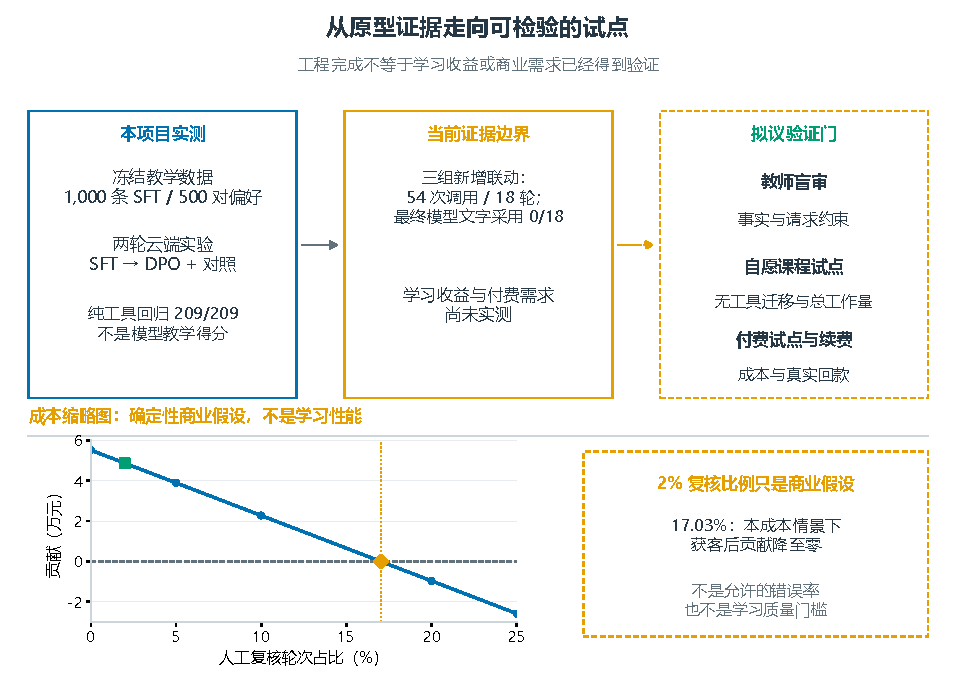
\includegraphics[width=\linewidth]{../../assets/zh/evidence-to-pilot.pdf}
\caption{从研究证据走向拟议受监督试点。实测、供应商公开说明和商业假设的证据作用不同；2\%复核是假设，17.03\%为成本边界，二者都不是实测质量或客户结果。}\label{fig:concise-business-evidence}
\end{figure}\FloatBarrier

\subsection{外部研究能说明什么}
教育部报告2025年高校3167所、高等教育在学规模4872.57万人，包含多种教育形式\cite{businessmoe}。缺少可核验的目标院系、Python 修课人数、预算和采购意愿，不能据此计算已验证市场规模。

Kestin 等的本科物理交叉研究为两周两课，233名选课者中194人纳入，专家设计的 AI 辅导在即时后测上获益\cite{businesskestin}；该系统特定结果不是本项目收益。Bastani 等在土耳其单所高中、近1000名学生的数学试验中发现，无保护 GPT Base 撤去工具后的考试成绩相对对照低约17\%，是相对变化而非百分点；带教学保护的 GPT Tutor 在对应考试结果上也未显示显著正增益\cite{businessbastani}。CodeAid 在700人的编程课程部署12周、分析约8000次交互，强调认知参与和避免直接代写\cite{businesscodeaid}。这些研究支持分别测量有辅助练习、无辅助迁移、延迟保持与教师工时，不能拼成产品排名或付费需求结论。

\section{竞品与差异化假设}
CodeGrade 直接覆盖编程提交、测试、反馈和教师流程；Khanmigo 是范围更广的导师及学校采购比较对象。选择依据是任务相关性，不是市场份额排名。表\ref{tab:concise-business-competitors}依据归档官方说明，未核实某功能不表示该功能不存在。

\begin{table}[htbp]\centering\small
\caption{官方公开能力与当前原型对照（2026年11月7日）。}\label{tab:concise-business-competitors}
\begin{tabularx}{\linewidth}{@{}p{23mm}Y Y Y@{}}\toprule
维度 & CodeGrade & Khanmigo & 本项目\\\midrule
范围 & 编程提交、测试、自动评分 & 跨学科导师、编程辅导、教师和学校方案 & Python 入门研究原型\\
教师与证据控制 & 按作业配置提示和助手；查看会话；代码及学生可见 AutoTest 上下文 & 教师工具和机构接入；本次未核实同类执行轨迹 & 受限解释器、原始审计日志；面板权限未实现\\
接入与记忆 & Advanced/机构方案有 LMS；可看历史，未核实相同主题计数 & 学校名册与单点登录；近期作业摘要，未核实相同计数 & 本地 SQLite；保留 S02 原故障和独立修复；无机构部署\\
采购 & 按课程计划、机构询价 & 免费教师工具、个人订阅、学校询价 & 拟议课程服务；无合同成交证据\\\bottomrule
\end{tabularx}
\par\smallskip\raggedright\scriptsize 来源：CodeGrade 官方价格、产品、帮助、版本说明\cite{businesscgprice,businesscgai,businesscghelp,businesscgrelease}；Khanmigo 价格和 FAQ\cite{businesskhanprice,businesskhan}。公开能力未经过同题账号实测。
\end{table}\FloatBarrier

CodeGrade 免费计划至多50人/课程；Starter 为\$24/学生/课程，Advanced 为\$39，AI 附加项\$15，机构询价\cite{businesscgprice}。读取正文未明确 ISO 币种与税费，保留官网“\$”而不折算人民币。帮助页仍称 Beta，2026年9月版本说明描述付费附加功能，权限须采购时确认\cite{businesscghelp,businesscgrelease}。Khanmigo 教师工具免费，个人/家庭\$4/月或\$44/年、不含销售税，学校询价\cite{businesskhanprice}；个人/家长入口要求成年、美国居住和账单地址，教师工具覆盖更广地区\cite{businesskhan,businesskhangeo}。两家对中国高校的合同、数据驻留和供货条件未核实；个人、课程与机构价格不能直接排序。

通用助手也是替代品。ChatGPT 学习模式公开说明包含免费入口、引导问题、可选记忆及错误和方案限制\cite{businessstudymode}；CodeGrade 已有教师可见和测试上下文。本项目应验证的差异因此是中文课程适配、查错和记录更正的\emph{总负担}是否更低，而非多智能体形式是否新颖。教师授权映射、核验错例和交付经验可能积累，但尚无技术壁垒；现有 LMS 加通用助手应作为实际替代方案比较。

\section{条件化商业模式与单位经济}
假设院系年合同覆盖每学期300人次、两学期共600个“学生--课程”人次，并非600名独立学生。每人次每学期120元，年合同72000元；用量封顶、超额、权限与接入须写入合同。获客拟按教师试点、教研认可、IT审查、预算采购推进；100个待筛院系、20个机会、10次演示、3份合同的漏斗尚无真实名录。年末三份合同对应21.6万元年化合同规模，不是当年到账或已确认收入。

若买方教师时间按90元/小时估值，7.2万元年费需净节省800小时、即每人次80分钟，才能仅靠省时覆盖；20分钟仅值1.8万元/年。这是估值算术，不是实测收益，未减少的固定工资不能当作现金节省。

\subsection{成本模型与压力条件}
假设每人次120轮反馈，\emph{三个角色合计}每轮4500输入、900输出 token，重试系数 $k=1.10$。单价参考百炼 qwen-plus 华北2（北京）、输入至128k、实时非思考公开原价：输入0.8元、输出2元/百万 token，不计优惠\cite{businessprice}。未测试该较大 API 模型的教学或延迟，它也不是第二章训练的0.5B模型。

令 $N$ 为年人次、$s$ 为每人次轮数，$T$ 为合计 token，$p$ 为单价，$r$ 为人工复核比例、$m$ 为分钟、$w$ 为外包时薪，则
\begin{align}
C_{\rm API}&=Nsk\frac{T_{\rm in}p_{\rm in}+T_{\rm out}p_{\rm out}}{10^6},\\
C_{\rm review}&=Nsr\frac{m}{60}w,\\
G&=NP-C_{\rm API}-C_{\rm review}-C_{\rm setup}-C_{\rm cloud}-C_{\rm acquisition}.
\end{align}
合计 token 已含三次调用，不能再乘三。$P$ 为每人次单价，$G$ 扣交付和增量获客、未扣公司固定费用，不是利润或全成本 CAC。基准为2\%复核、每次3分钟、90元/小时、接入80小时、专属云每年1200元、每份新合同获客8000元。变动外包工时不重复计入固定工资；这些数值均不是询价结果。

\begin{figure}[htbp]\centering
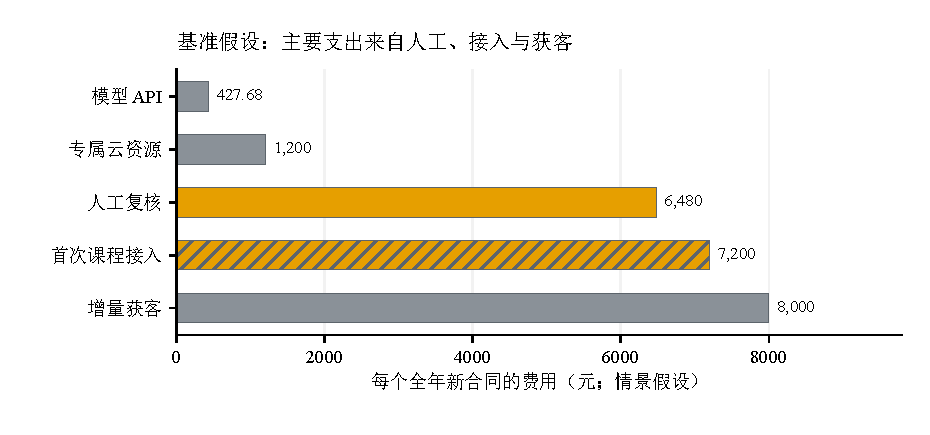
\includegraphics[width=\linewidth]{../../assets/zh/business-costs.pdf}
\caption{基准假设下全年单合同费用。API 为外部单价乘假设用量，人工、接入、云与获客均为规划输入；公司固定费用另计。}\label{fig:concise-business-costs}
\end{figure}\FloatBarrier

\begin{table}[htbp]\centering\small
\caption{基准与联合压力假设。金额为元/全年新合同；完整输入和效率情景保留于补充数据。}\label{tab:concise-business-finance}
\begin{tabularx}{\linewidth}{@{}Yrr@{}}\toprule
项目 & 基准 & 联合压力\\\midrule
每人次单价；每人次轮数 &120；120&90；180\\
复核比例；每次分钟 &2\%；3&5\%；5\\
全年收入 &72000&54000\\
交付成本 &15307.68&54072\\
增量获客 &8000&15000\\
扣交付与获客后贡献 &48692.32&$-15072$\\\bottomrule
\end{tabularx}
\end{table}\FloatBarrier

基准交付包括 API 427.68元、复核6480元、接入7200元、云1200元，扣获客前直接贡献率78.74\%。联合压力还假设接入120小时、云1800元，扩张不能挽救其负贡献。固定支出每年60万元（每月5万，其中人员4.2万），需13份基准全年合同覆盖，连同10万元启动费则需15份；静态全年计算不能当作年中陆续启用的第一年。没有给情景赋概率，也不推算终身价值和续费。

\begin{figure}[htbp]\centering
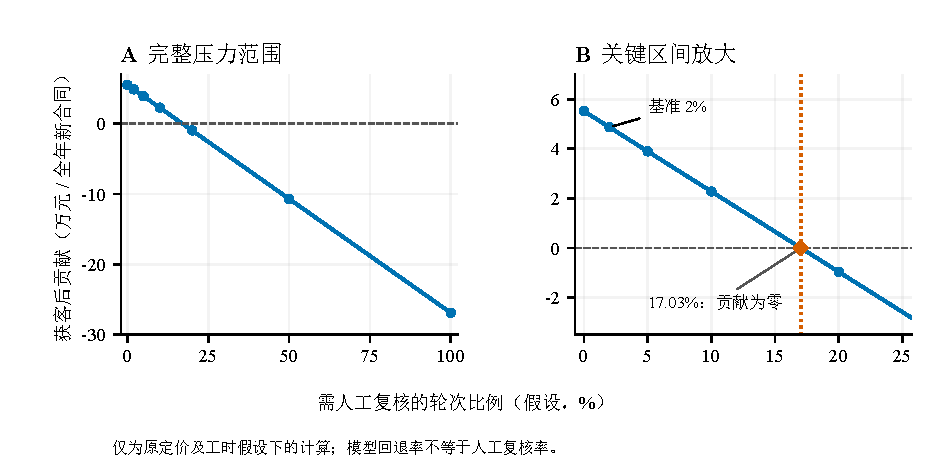
\includegraphics[width=\linewidth]{../../assets/zh/business-review-stress.pdf}
\caption{其余基准不变时的人工复核敏感性。约17.03\%的零贡献点是商业承受边界，不是可接受质量门槛或实测复核率。}\label{fig:concise-business-review}
\end{figure}\FloatBarrier

复核比例10\%、20\%、50\%时，年贡献分别为22772.32、$-9627.68$、$-106827.68$元。模型不采用或回退频次不能直接折算为业务复核概率。若达到质量要求的人工负担超过17.03\%盈亏边界，应调价、缩小范围或停止产品化，不能为了毛利削弱质量保护。

\subsection{现金计划与模拟融资}
模拟融资100万元，支持十二个月工程、试点和采购验证，不设未经依据的估值或退出回报。年合同于第4、7、10月启用，启用时开票，三个月后回款；收入按服务月份摊分，只是规划口径。计划包含首月10万元启动费、每月5万元固定支出，以及启用时的接入获客和使用成本；真实获客费用可能更早发生。

\begin{figure}[htbp]\centering
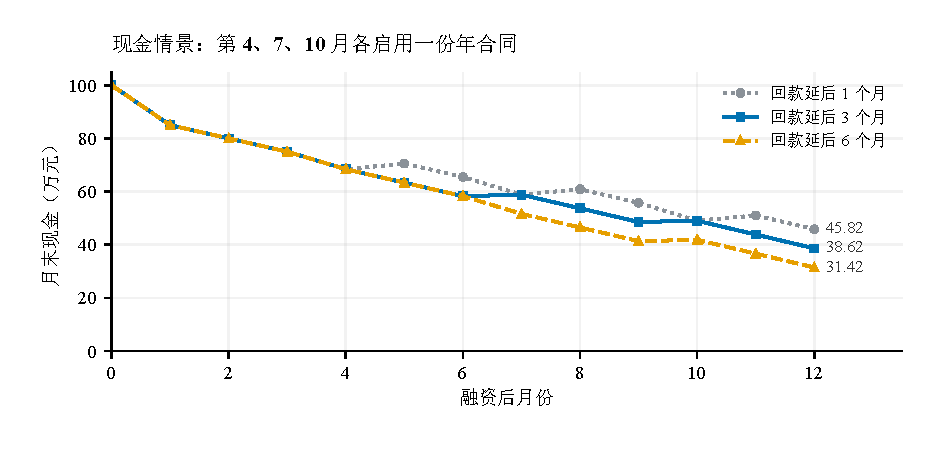
\includegraphics[width=\linewidth]{../../assets/zh/business-cash.pdf}
\caption{融资100万元、分别延迟1、3、6个月回款的现金情景。合同启用与收款均未实际发生。}\label{fig:concise-business-cash}
\end{figure}\FloatBarrier

三个月回款基准首年分摊收入10.8万元、到账14.4万元、年末年化合同21.6万元；支出约75.78万元，余额38.62万元，第10月合同第二年回款。余额须支持后续履约，不是利润。税费、融资、坏账、退款和硬件未计；智能体研究 本机时长不能代表生产延迟或云容量。试点推迟须重算现金流。

\section{验证门槛与决策}
下一步应在补充内容核验后开展受监督试点，而非按日期自动销售。C08/S02 已知输入的工程修复完成；独立教师审阅、学生收益和采购验证尚未开展。

\begin{table}[htbp]\centering\small
\caption{拟议采集与放行条件，均为计划而非已获结果。}\label{tab:concise-business-gates}
\begin{tabularx}{\linewidth}{@{}p{29mm}Y@{}}\toprule
阶段 & 证据与决策边界\\\midrule
内容核验 & 新独立题集和100条教师盲审；严重错误零例才放行，严重误导、越权或记忆污染立即暂停。\\
课程试点 & 两门课约100名自愿学习者，尽量课内随机；计入全部备题、复核、纠错和维护工时，两周后无辅助迁移、盲化阅卷。用于可行性和方差，不保证统计效力。\\
质量与工作量 & 拟议误导率 $\leq2\%$、净节时 $\geq20\%$、后测相对对照不低于 $-5$ 分（满分100）。预登记并报区间，跨门槛视为不确定；独立100条零误导的单侧95\%上界仍为2.95\%；支持2\%误导率门槛至少需149条独立且零误导的审查，同一学生的多条记录未必独立。\\
采购与交付 & 访谈15名教师、5名采购角色；演示前记录现流程，区分拒绝、报价、签约、开票和到账。3个合作意向是目标，不是3个已有客户。\\\bottomrule
\end{tabularx}
\end{table}\FloatBarrier

仅靠20\%净节时抵付假设费用，原工作量须至少达到每人次400分钟；目前尚未测量，否则应调整价格或另证其他收益。严重事件与一般误导率单列。试点需与教师确定门槛，记录交流污染、退出，并用现有课程支持作对照。团队需要工程、课程评价和客户交付职责，不代表已招募人员或建立校方合作。

学生标识和错误历史的未来处理需明确依据、最小字段、期限、更正删除、委托职责和必要影响评估\cite{businesspipl}。伪名、课程权限和更正审计是拟议要求，不是已经完成的合规认证。生产还需代码隔离、并发安全测试、供应商版本和采购数据条款核实。免费替代、适配工时、延期和续费仍有风险；若只能靠密集人工保证质量，应按服务业务如实报价，负贡献则停止扩张。

证据支持有限的受监督验证准备，不支持自主教学、竞品优势或已验证付费意愿。完整网页副本、21项来源台账、三种财务情景、25组敏感性、逐月现金、访谈审查表和计算代码保留在 \path{business/}、\path{business/validation/}。

\paragraph{阅读提示（不属于新实验）。}
“算得出来”只是模型在假设下自洽，不代表有人会买；收入、到账和利润也不是同一件事。特别要看复核人工是否吞掉贡献，以及教师实际省下的时间能否支持价格。图中的17.03\%是成本算出的边界，不能反过来当成教学质量标准。
\FloatBarrier
\begin{thebibliography}{99}
% report opens the bibliography with \chapter*. hyperref sets the heading's
% destination there; writing the entry now keeps the TOC link on that page.
\addcontentsline{toc}{chapter}{\bibname}
\small
\setlength{\itemsep}{4pt}

\bibitem{nat}
Yang Li, Youssef Emad, Karthik Padthe, et~al.
\href{https://arxiv.org/abs/2507.01921v1}{NaturalThoughts: Selecting and Distilling Reasoning Traces for General Reasoning Tasks}.
arXiv:2507.01921v1, 2025.

\bibitem{matrix}
Dong Wang, Yang Li, Ansong Ni, et~al.
\href{https://arxiv.org/abs/2511.21686v2}{Matrix: Peer-to-Peer Multi-Agent Synthetic Data Generation Framework}.
Conference on Machine Learning and Systems (MLSys), 2026. This report uses arXiv:2511.21686v2.

\bibitem{air}
Bingxiang He, Wenbin Zhang, Jiaxi Song, et~al.
\href{https://openreview.net/pdf?id=Sz3ZU6oeVJ}{AIR: A Systematic Analysis of Annotations, Instructions, and Response Pairs in Preference Dataset}.
Conference on Language Modeling (COLM), 2025.

\bibitem{easy}
ConardLi and contributors.
\href{https://github.com/ConardLi/easy-dataset}{Easy Dataset}.
GitHub repository, accessed 4 November 2026.

\bibitem{dataflow}
OpenDCAI and contributors.
\href{https://github.com/OpenDCAI/DataFlow}{DataFlow}.
GitHub repository, accessed 4 November 2026.

\bibitem{trl}
Hugging Face.
\href{https://huggingface.co/docs/trl/en/dataset_formats}{Dataset formats and types}.
TRL documentation, accessed 4 November 2026.

\bibitem{fdpo}
Tetsuro Morimura, Mitsuki Sakamoto, Yuu Jinnai, Kenshi Abe, and Kaito Ariu.
\href{https://aclanthology.org/2024.emnlp-main.1266/}{Filtered Direct Preference Optimization}.
Proceedings of EMNLP, 2024, pp.~22729--22770.

\bibitem{rethink}
Ziche Liu, Rui Ke, Yajiao Liu, Feng Jiang, and Haizhou Li.
\href{https://aclanthology.org/2025.naacl-long.336/}{Take the Essence and Discard the Dross: A Rethinking on Data Selection for Fine-Tuning Large Language Models}.
Proceedings of NAACL, Volume~1: Long Papers, 2025, pp.~6595--6611.

\bibitem{deita}
Wei Liu, Weihao Zeng, Keqing He, Yong Jiang, and Junxian He.
\href{https://openreview.net/forum?id=BTKAeLqLMw}{What Makes Good Data for Alignment? A Comprehensive Study of Automatic Data Selection in Instruction Tuning}.
International Conference on Learning Representations (ICLR), 2024.

\bibitem{learnlm}
Irina Jurenka, Markus Kunesch, Kevin R.~McKee, et~al.
\href{https://arxiv.org/abs/2407.12687v4}{Towards Responsible Development of Generative AI for Education: An Evaluation-Driven Approach}.
arXiv:2407.12687, 2024. The supplied v4 revision is used.

\bibitem{edu_survey}
Shen Wang, Tianlong Xu, Hang Li, et~al.
\href{https://arxiv.org/abs/2403.18105v2}{Large Language Models for Education: A Survey and Outlook}.
arXiv:2403.18105v2, 2024.

\bibitem{agent_survey}
Zhendong Chu, Shen Wang, Jian Xie, et~al.
\href{https://aclanthology.org/2025.findings-emnlp.743/}{LLM Agents for Education: Advances and Applications}.
Findings of the Association for Computational Linguistics: EMNLP 2025, pp.~13782--13810.
The supplied local version is \href{https://arxiv.org/abs/2503.11733v2}{arXiv:2503.11733v2}, revised 2026.

\bibitem{simclass}
Zheyuan Zhang, Daniel Zhang-Li, Jifan Yu, et~al.
\href{https://aclanthology.org/2025.naacl-long.520/}{Simulating Classroom Education with LLM-Empowered Agents}.
Proceedings of NAACL, Volume~1: Long Papers, 2025, pp.~10364--10379.

\bibitem{qwenbase}
Qwen Team. \href{https://huggingface.co/Qwen/Qwen2.5-0.5B}{Qwen2.5-0.5B: Base model card}. Official pretrained model and tokenizer configuration. \href{https://modelscope.cn/models/Qwen/Qwen2.5-0.5B}{official ModelScope repository}.

\bibitem{lora}
Edward J. Hu, Yelong Shen, Phillip Wallis, et al.
\href{https://arxiv.org/abs/2106.09685}{LoRA: Low-Rank Adaptation of Large Language Models}. ICLR 2022.

\bibitem{dpo}
Rafael Rafailov, Archit Sharma, Eric Mitchell, et al.
\href{https://arxiv.org/abs/2305.18290}{Direct Preference Optimization: Your Language Model is Secretly a Reward Model}. NeurIPS 2023.
\bibitem{openmaic}
THU-MAIC. \href{https://github.com/THU-MAIC/OpenMAIC/tree/5bd8cc840ee6397d063e1fe6aba974b9f0401593}{OpenMAIC: Open Multi-Agent Interactive Classroom}. GitHub repository, pinned commit \texttt{5bd8cc840ee6} (6 November 2026), accessed 7 November 2026. Full commit and file hashes:  \filepath{tutor/legacy/research/source_manifest.json}.

\bibitem{businesscambridge} Accelerate Cambridge. \href{https://www.jbs.cam.ac.uk/wp-content/uploads/2020/08/how-to-write-a-business-plan.pdf}{How to write a business plan}. Cambridge Judge Business School, October 2013. Business-plan reference supplied in the course specification.
\bibitem{businessmoe} Ministry of Education of the People's Republic of China. \href{https://www.moe.gov.cn/jyb_sjzl/sjzl_fztjgb/202607/t20260706_1442870.html}{Statistical Bulletin on National Education Development in 2025}. 6 July 2026. Cross-checked against the \href{https://jyt.hlj.gov.cn/jyt/c110518/202608/c00_31969727.shtml}{official Heilongjiang education-department republication}.
\bibitem{businesskestin} Greg Kestin, Kelly Miller, Anna Klales, Timothy Milbourne, Gregorio Ponti. \href{https://doi.org/10.1038/s41598-025-97652-6}{AI tutoring outperforms in-class active learning: an RCT introducing a novel research-based design in an authentic educational setting}. Scientific Reports 15, 17458, 2025. \href{https://pmc.ncbi.nlm.nih.gov/articles/PMC12179260/}{full text at PMC}.
\bibitem{businessbastani} Hamsa Bastani, Osbert Bastani, Alp Sungu, et al. \href{https://doi.org/10.1073/pnas.2422633122}{Generative AI without guardrails can harm learning: Evidence from high school mathematics}. PNAS 122(26), e2422633122, 2025. \href{https://pmc.ncbi.nlm.nih.gov/articles/PMC12232635/}{full text at PMC}.
\bibitem{businesscodeaid} Majeed Kazemitabaar, Runlong Ye, Xiaoning Wang, et al. \href{https://arxiv.org/abs/2401.11314v2}{CodeAid: Evaluating a Classroom Deployment of an LLM-based Programming Assistant that Balances Student and Educator Needs}. CHI 2024, DOI: 10.1145/3613904.3642773. The supplied arXiv v2 was checked.
\bibitem{businesscgprice} CodeGrade. \href{https://www.codegrade.com/pricing}{Pricing \& Plans}. Official dynamic pricing page, accessed 7 November 2026. Original units retained; not an institutional contract quote.
\bibitem{businesscgai} CodeGrade. \href{https://www.codegrade.com/solutions/ai-assistant}{AI Coding Assistant for CS Courses}. Official product description, accessed 7 November 2026.
\bibitem{businesscghelp} CodeGrade. \href{https://help.codegrade.com/setup-assignment/other-features/ai-assistant}{AI Assistant}. Official documentation, accessed 7 November 2026; the archived page retains a Beta description.
\bibitem{businesscgrelease} CodeGrade. \href{https://www.codegrade.com/blog/codegrade-snowball-miracle-release}{Snowball Miracle: A Terminal, a Smarter AI Assistant, and Tighter Exam Controls}. 25 September 2026; accessed 7 November 2026.
\bibitem{businesskhanprice} Khan Academy. \href{https://khanmigo.ai/pricing}{Khanmigo pricing}. Official dynamic pricing page, accessed 7 November 2026.
\bibitem{businesskhan} Khan Academy. \href{https://khanmigo.ai/}{Khanmigo: AI-powered teaching assistant \& tutor}. Official product and FAQ, accessed 7 November 2026.
\bibitem{businesskhangeo} Khan Academy. \href{https://blog.khanacademy.org/teachers-in-44-countries-now-get-free-access-to-khanmigo-in-english-thanks-to-microsoft-support/}{Khanmigo for Teachers Now Available in Pilot in 180+ Countries, Powered by Microsoft}. Initially published 17 July 2024, explicitly updated 4 December 2025; accessed 7 November 2026.
\bibitem{businessstudymode} OpenAI. \href{https://help.openai.com/en/articles/11780217-using-study-mode-in-chatgpt}{Using study mode in ChatGPT}. Official help page, accessed 7 November 2026; availability and limits depend on plan, region and updates.
\bibitem{businessprice} Alibaba Cloud. \href{https://help.aliyun.com/zh/model-studio/qwen-plus}{qwen-plus model information}. China North 2 (Beijing), input up to 128k, real-time non-thinking list price; accessed 7 November 2026. No discount or teaching-effect claim.
\bibitem{businesspipl} Standing Committee of the National People's Congress. \href{https://www.cac.gov.cn/2021-08/20/c_1631050028355286.htm}{Personal Information Protection Law of the People's Republic of China}. Adopted 20 August 2021, effective 1 November 2021; CAC republication, accessed 7 November 2026.

\end{thebibliography}

\appendix\renewcommand{\chapterprefix}{附录\thechapter}
\chapter{证据与复现}\label{app:repro}\section{发布证据与复现边界}
仓库提供源码、冻结教育数据、保存的回答与逐题审阅。报告构建不重新运行数值实验。官方模型、适配器和优化器二进制、本机运行环境不随仓库分发；重新运行模型需固定官方基座与说明中的依赖。查看已存结果无需模型推理。
\begin{table}[htbp]\centering\small
\caption{研究证据与代码入口。}
\begin{tabularx}{\linewidth}{@{}p{27mm}Y@{}}\toprule
领域 & 发布文件\\\midrule
数据合成 & \filepath{synthesis/}：生成器、1000条SFT和500对偏好、候选账本及核验；\filepath{synthesis_legacy/}、\filepath{data/legacy/}保留早期筛选对照。\\
后训练 & \filepath{training/}：SFT/DPO与评估代码、两轮云端结果、继续SFT对照、完整回答、初次失败的数值审计及独立复审。\\
学生记忆 & \filepath{tutor/}：冻结案例、修订与结构化控制器、角色原文、记忆证据、工具回归及隔离的输出修复。\\
可行性 & \filepath{business/}：来源、商业假设、单位经济、敏感性及待执行的验证计划。\\
科研图 & \filepath{reports/assets/}：矢量科研图与概念插画；后者不属于实验测量。\\\bottomrule
\end{tabularx}\end{table}\FloatBarrier
英文摘录是中文实录的翻译，不是新的英文模型评估；事实判断仍依据完整原回答。发布记录删除身份与本机字段，保留科学数值和失败标签。历史运行散列描述原始实验文件，发布清单另行核对仓库文件。

两语说明提供依赖、已存记录核对、不加载模型的控制器检查，以及可选训练命令。重建PDF需Tectonic或兼容XeLaTeX与说明中的字体。能够运行流程不等于已经验证自主教学能力或真实学生学习收益。
\FloatBarrier
\chapter{研究来源与局限}\label{app:prompts}\section{模型辅助与证据边界}
OpenAI Codex/GPT-6系列辅助研究、代码、审阅、翻译和科研图设计。被研究的是官方Qwen2.5-0.5B基础模型与记录的适配器；另行获取的同规模Instruct只作诊断，不算训练成果。规则合成没有逐条调用教师模型；技术审阅来自同一项目且非盲化，不属于独立教师评价。

研究角色模板与记录的模型输入随控制器和运行证据提供。匿名发布不包含个人对话及内部任务分工历史，也不声称提供全部写作提示。科研示意图由可编辑代码生成；OpenAI图像工具生成无字概念封面，工具未返回精确生成模型标识。

\section{局限}
数据限于Python子集，模板重复、偏好理由与任务类型有关联；开发和评估题较少、同源编写，仅单训练种子，追加研究复用已观察测试，对照token预算不匹配。这些条件限制因果归因；没有更大模型或数据控制消融。参考NLL、解析成功和回退正确都不等于学习收益。系统信任调用者传入学生ID，尚无生产身份认证。真实学生收益、教师工时节省、机构需求和付费意愿均未实测；失败回答、原数值异常和有限补救失败继续保留。

\end{document}
